\chapterimage{head2.png} % Chapter heading image
\chapter{Magnification in DES}
\label{ch:magnification}

Extensive wide-field programs have allowed accurate measurements of weak-lensing effects. Previous magnification measurements involve the use of very massive objects as lenses, such as luminous red galaxies (LRGs) and clusters \cite{1995AIPC..336..320B,2014MNRAS.440.3701B,2014MNRAS.439.3755F,2016MNRAS.457.3050C}, or high redshift objects as sources, such as Lyman break galaxies (LBGs) \cite{2009A&A...507..683H,2012MNRAS.426.2489M}, quasars (QSOs) \cite{1979ApJ...227...30S,1989Natur.339..106H,1990A&A...240...11F,1993A&A...268....1B,2002A&A...386..784M,0004-637X-633-2-589} and sub-mm sources  \cite{2011MNRAS.414..596W} to improve signal-to-noise ratio. In addition to the number count technique used on this Thesis, other observational effects produced by magnification have been measured as well: the shift in magnitude \cite{2010MNRAS.405.1025M}, flux \cite{2011MNRAS.411.2113J} and size \cite{2041-8205-780-2-L16}.
\newline

On this chapter, first, the methodology to measure magnification is described (\autoref{sec:method}) and validated with simulations (\autoref{sec:mice}). Then, the methodology is used to measure the magnification signal at the Dark Energy Survey Science Verification data (SV; \autoref{sec:svdata}). Finally, the same technique used at the DES-SV data is employed to measure the convergence profile of voids and troughs with the Year 1 data (Y1; \autoref{sec:y1data}).
\newline

It is worth to remark that, as it has been defined at \autoref{ch:theory}, given both the redshift of the lenses and the sources, the convergence is a two-dimensional scalar field that is independent on the selected lens or source sample. Nevertheless, by choosing the suitable lens sample, different parts of the log-normal distribution of the convergence field \cite{2017MNRAS.466.1444C} can be probed, leading to a different convergence profile.

\section{Measuring Magnification through Number Count}
\label{sec:method}
As it has been described at \autoref{ch:theory}, the amplitude of the magnification signal is dependent on two factors: the number-count slope parameter ($\alpha-1$) and the lensing kernel, that for a given lens sample, depends on the redshift of the source sample. LBGs and QSOs has been traditionally used on magnification studies as sources since they have an steep magnitude distribution, leading to a high value of $\alpha-1$. In addition, this population of galaxies is located at very high redshift ($2\lesssim z\lesssim 4$), leading to a high lensing efficiency and a clean redshift separation between the lens and source sample. Nevertheless, this population of galaxies has much less density than the general population of galaxies, feature that can prevent the measurement of a magnification signal for low-area surveys. In addition, the selection of a population of LBGs involve the known as {\it dropout} technique, that requires the development of a custom data-reduction pipeline just to select this specific population of galaxies. For large-area surveys such as DES and LSST, the amount of computing time to run the data-reduction pipeline is enormous ($\sim 1$ year), reaching manpower and infrastructure limitations.
\newline

The caveats related to the use of LBGs and QSOs as sources can be avoided by selecting galaxies from the general population of galaxies, that is, not selecting an specific subset of the full sample of galaxies. Then, only redshift cuts are imposed in order to separate the lens and source samples. This approach has the advantage that the density of the source sample is more populated, reducing significantly the shot-noise. Nevertheless, the accuracy on the determination of the redshift on broad-band galaxy-surveys --such as DES-- is very limited, introducing an important source of systematic errors that must be avoided and carefully taken into account.
\newline

In addition to the lens-source redshift overlap, magnification suffers from several systematic errors based on the photometry \cite{2015MNRAS.454.3121M,2016MNRAS.455.3943H}, such as: depth-inhomogeneities, patchiness of the zero-point correction and calibration, or shifts on the magnitude determination due to wrong sky-background subtraction. The important reduction of shot-noise on wide-field surveys requires the development of new techniques to estimate these systematic errors.
\newline

The use of the general population of galaxies on shallow small-area surveys is mandatory to reach a significance that allows the detection of the magnification signal. On wide-area surveys the use of this population is not necessary although new studies can be made if it is used. Having a very dense population of galaxies as sources allows to use a set of lenses that are less numerous: voids and troughs. This allows to produce new physics analysis.
\newline

The usual approach that can be found on the literature to measure magnification the {\it optimal weighting} technique \cite{2003A&A...403..817M}. This methodology can be summarized as follows:
\begin{enumerate}
\item Split data sample into two well-separated photo-z bins, termed lens and source. Splitting must be done minimizing the overlap between the true redshift distributions of the samples. Otherwise, by \autoref{eq:4t}, an additive signal is introduced.
\item Weight each source galaxy by its {\it optimal weight}.
\item Compute the two-point angular cross-correlation between the lens and the unique source sample.
\end{enumerate}
The weight of the $i$-th galaxy ($w_i$) is given by:
\begin{equation}
w_i = \alpha_S(m_i)-1,
\end{equation}
where $\alpha_S(m_i)$ is the number-count slope given by \autoref{eq:alpha} and $m_i$ is the magnitude of the $i$-th galaxy. This procedure allows to obtain the maximum signal-to-noise. Nevertheless, this weighting makes hard to model the impact of the different systematic effects on the measured signal.
\newline

As an alternative approach the following procedure is proposed:
\begin{enumerate}
	\item Split the data sample into two well-separated photo-z bins, termed lens and source. Splitting must be done minimizing the overlap between the true redshift distributions of the samples. Otherwise, by \autoref{eq:4t}, an additive signal is introduced.
	\item For each photometric band, define several subsamples from the source sample using different values for the maximum (threshold) magnitude. This is made in order to trace the evolution of the amplitude of the magnification signal with the number count slope (see \autoref{eq:alpha}).
	\item Compute the two-point angular cross-correlation function between the unique common lens sample and each source subsample for each band.
\end{enumerate}
Once the two-point angular correlation function has been measured, it can be compared with theoretical predictions as described in \autoref{ch:theory} allowing the desired parameter constraints.
\newline

As has been stated previously, the amplitude of the measured cross-correlation function depends on the shape of the galaxy number count distribution. Nevertheless, due to this shape --for a fixed footprint, population of galaxies and redshift distribution--, the brighter is the magnitude limit of the sample, the bigger is the amplitude of the two point angular cross correlation function. However, the number of bright galaxies is lower than the number of faint galaxies \cite{1976ApJ...203..297S}, so shot noise is bigger at brighter magnitude cuts, increasing their measurement uncertainties. For this reason, there exists a magnitude cut that is a trade-off between amplitude and shot noise, maximizing the signal-to-noise ratio.  In  order to find the optimum magnitude cut for a given sample, define the signal-to-noise ratio for a given angular range  and magnitude cut $m'<m$ as \cite{1998MNRAS.294L..18M}:
\begin{equation}
\frac{S}{N}(m) = \frac{\langle \omega_{LS}(\theta;m)\rangle}{\langle s(\omega_{LS}(\theta;m))\rangle},
\label{eq:sn}
\end{equation}
where $\langle s(\omega_{LS}(\theta;m))\rangle$ is the average shot noise of the two point angular cross correlation functions and the averages are extended to the angular range considered in the analysis. The shot noise for a given angular aperture is given by the number of pairs inside each angular bin as
\begin{equation}
\sigma(\omega_{LS}(\theta;m)) = \frac{1}{\sqrt{P_{LS}(\theta;m)}},
\end{equation}
where $P_{LS}(\theta;m)$ is the number of pairs from the lens-source samples separated by an angular distance $\theta$ for a magnitude cut $m '<m$. The number of pairs per angular bin is given by the product of the number of source galaxies that fall inside a given annulus times the number of sources inside that annulus. Considering, as a first order approach, that the samples are uniform, the number of lens-source pair-counts of galaxies for a bin centerd at $\theta$ with solid angle $\Delta_\Omega$ is given by
\begin{equation}
P_{LS}(\theta;m) = \left[\frac{N_L}{A}\Delta_\Omega(\theta)\right]\left[\frac{N_S(m)}{A}\Delta_\Omega(\theta)\right].
\label{eq:PLS}
\end{equation}
Here $A$ is the solid angle subtended by the dataset, $N_L$ is the number of objects at the lens sample and $N_S(m)$ the number of objects on the source sample with magnitude limit $m$. Combining Equations \ref{eq:numbercountstheo}, \ref{eq:sn} and \ref{eq:PLS}, results finally in
\begin{equation}
\frac{S}{N}(m) = \langle\omega_0\rangle[\alpha(m)-1]b_L\frac{\Omega}{A}\sqrt{N_LN_S(m)},
\label{eq:snfinal}
\end{equation}
where $\Omega$ is the solid angle subtended by an annulus with edges the maximum and minimum scales considered. Thus, for a sample, given size, magnitude and redshift distributions --assuming a cosmology-- the signal-to-noise ratio can be estimated. Nevertheless, \autoref{eq:snfinal} assumes that the angular bins are uncorrelated and should be taken as an upper bound to the signal-to-noise. Although this expression does not take into account the full covariance, the behavior
\begin{equation}
\frac{S}{N} \sim [\alpha(m)-1]\sqrt{N_S(m)},
\label{eq:maxsn}
\end{equation}
is independent of cosmological and covariance assumptions up to a constant factor, allowing us to use this expression for finding the optimal cut that maximizes the signal-to-noise ratio.
\newline

\autoref{eq:maxsn} finds the magnitude cut with the maximum signal-to-noise for a given source sample. Nevertheless, this requires the use of less data than the {\it optimal weighting } approach, reaching a lower significance since less information is used. To overcome this, all the magnitude cuts within a band --not just the maximum-- are used, tracing the number-count slope evolution.

\section{Magnification in the MICE-GC simulation}
\label{sec:mice}
\begin{sidewaysfigure}
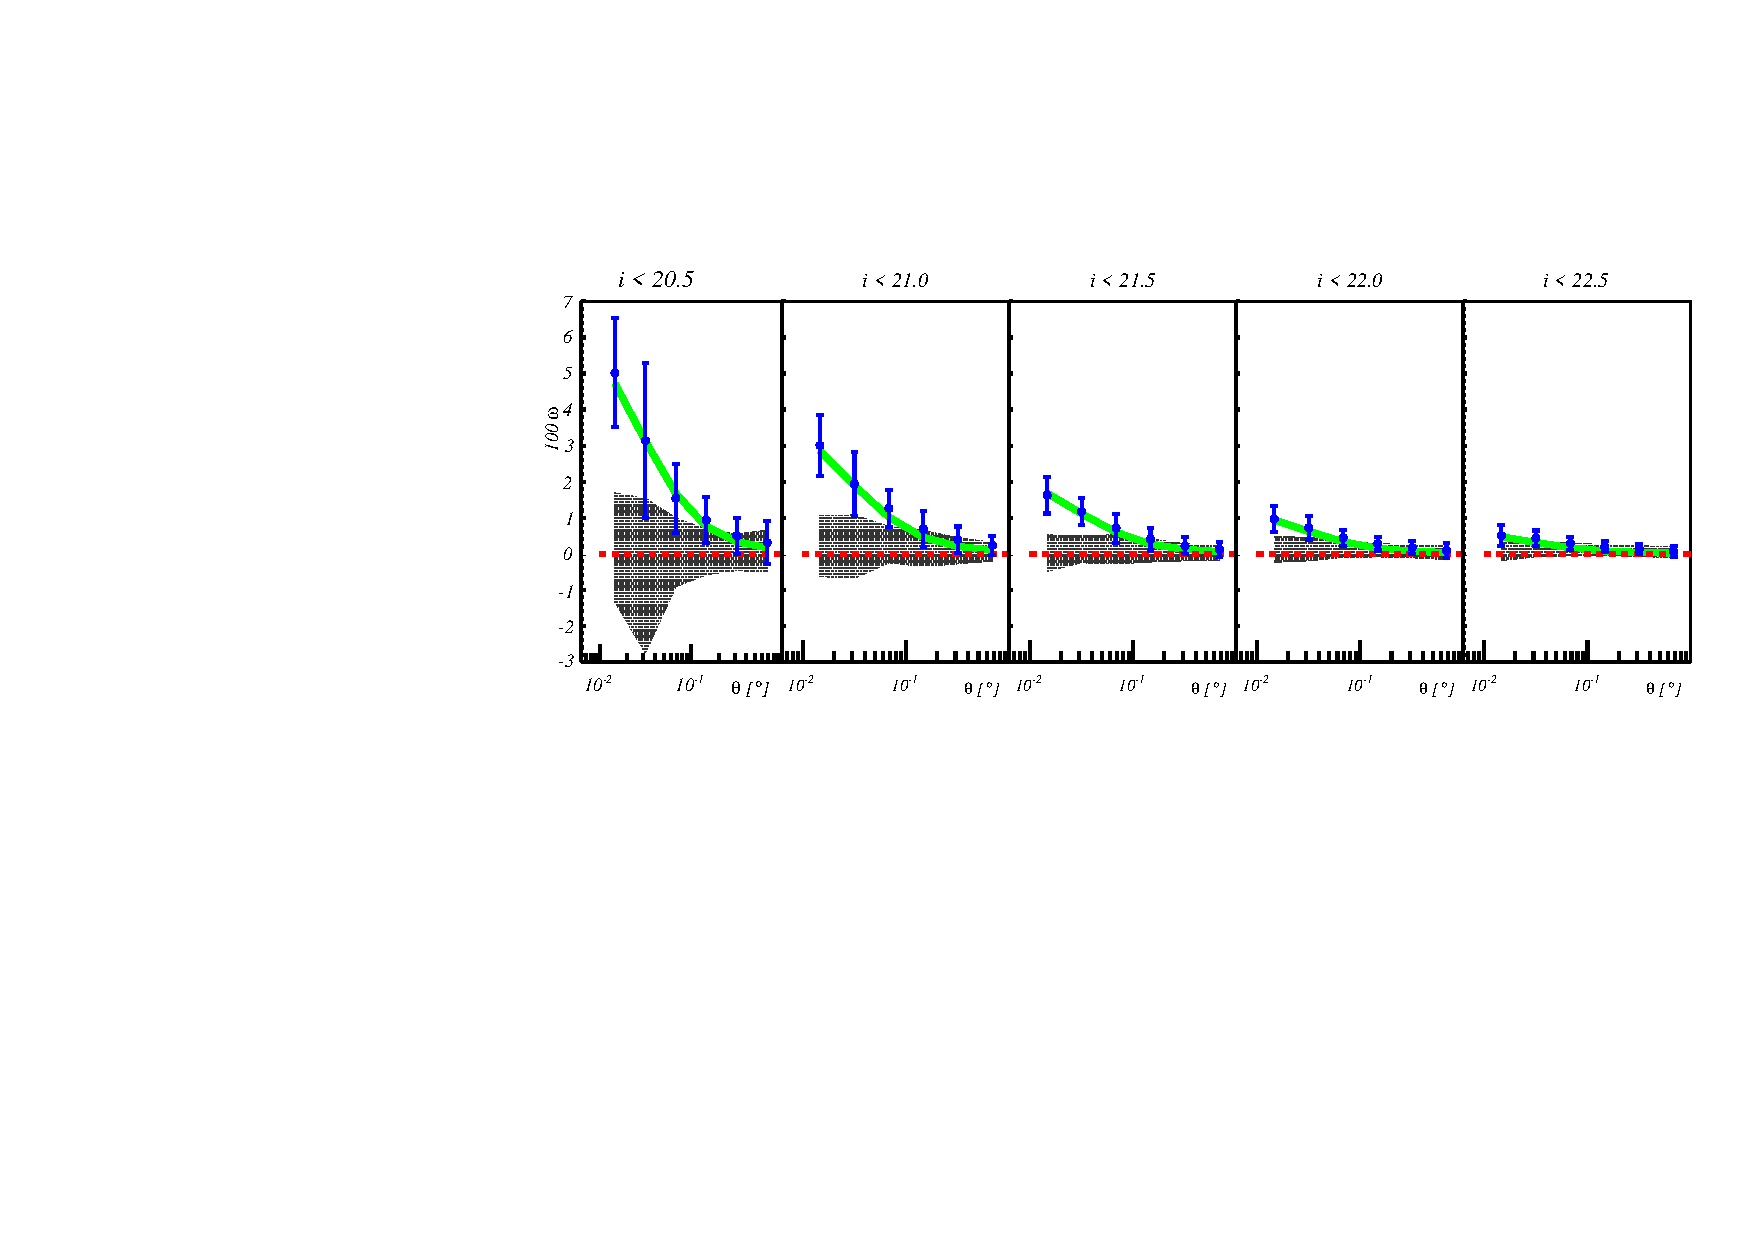
\includegraphics[width=\textwidth,trim={0 2.3cm 0 3.5cm},clip]{./figures/mag_i_MICE.pdf}
\caption{Two-point angular cross-correlation functions for the MICE simulation (sample $i < 21.5$): measured, both with magnification (blue dots) and without (grey shade), versus that expected from the MICE cosmological parameters, both with magnification (green solid line) and without (red dashed line), the latter being zero.}
\label{fig:MICE}
\end{sidewaysfigure}
In order to test the methodology described above in a controlled environment, isolated from any source of systematic error, it is applied to a simulated galaxy sample, in particular {\scshape MICECAT v1.0}.
This mock is the first catalog release of the N-body simulation MICE-GC\footnote{www.ice.cat/mice} \cite{2015MNRAS.447.1319F,2015.2987F,2015MNRAS.453.1513C}. It assumes a flat $\Lambda$CDM Universe with cosmological parameters $\Omega_M=0.25, \Omega_b=0.044, h=0.7$ and $\sigma_8 = 0.8$, using a light-cone that spans one eighth of the celestial sphere. Another advantage of using these simulations is the possibility of studying specific systematic effects, as described in \autoref{sec:sys}.

Among other properties, MICE-GC provides lensed and unlensed coordinates, true redshift (including redshift space distortions) and DES-$griz$ unlensed magnitudes for the simulated galaxies, along with convergence and shear.
Conversion from unlensed magnitudes to lensed magnitudes can be done by applying $m_\mu = m_0-2.5\log_{10}(1+2\kappa)$.

Having two sets of coordinates and magnitudes, one in a `universe' with magnification and another without magnification, allows us to follow the methodology described in \autoref{sec:method} for both cases,
serving as a test-bench to measure the sensitivity of the method to the magnification effect. In order to have a fiducial function with as little statistical uncertainty as possible, the full 5000 deg$^2$ of the MICE simulation are used. To match as much as possible the conditions of the DES-SV data, the magnitude cuts described in \autoref{sec:data_sample_SV} are applied to the lens and source samples. The covariance matrices of data (see \autoref{sec:svdata}) are used, in order to match the errors in the DES-SV sample.

In \autoref{fig:MICE}, the results of the magnification analysis in the MICE simulation for the cases with and without magnification can be seen compared with the theoretical expectations. The methodology used in this work clearly allows us to distinguish both cases for a data-set similar to that of the DES-SV data. Nevertheless, results obtained with the MICE simulation can not be directly extrapolated to SV data to estimate the expected significance because the density of galaxies on the simulation is a factor $\sim3$ smaller than on the SV data. Also, the luminosity function of the simulation is slightly different from the DES data, which has a direct impact on the number count slope and, consequently, on the amplitude of the measured signal.


\section{Magnification in DES Science Verification data}
\label{sec:svdata}
As of January 2014 --when I started my PhD--, the only data available at DES was the Science Verification data. The first data-release from DES. This data were taken just for testing purposes and in order to explore the capabilities of the experiment. Thus, although the nominal depth of the survey was reached, only $\sim 150$ deg$^2$ where taken. Taking this into account, only $10^4$ LBGs are expected at the full DES-SV data, preventing the measurement of magnification with the usual approach. Thus, in order to be capable to reach a detection of the magnification signal with the DES-SV data, the general population of galaxies was selected both as lens and source sample.
\newline

The goal of this analysis is to detect a weak-lensing magnification signal and develop methodology to mitigate systematic errors. Data sample is described at \autoref{sec:data_sample_SV}. Then, the analysis is described and the results discussed at \autoref{sec:analysis_sv} following the analysis of the possible systematic errors on \autoref{sec:sys}. Finally a discussion on the analysis can be found at \autoref{sec:discussion_sv}.

\subsection{Data sample}
\label{sec:data_sample_SV}
From the DES SVA1-Gold\footnote{des.ncsa.illinois.edu/releases/SVA1} main galaxy catalog \cite{2016MNRAS.455.4301C}, the largest contiguous field is selected, the SPT-E. Regions with declination $ < -61^{\circ}$ are removed in order to avoid the Large Magellanic Cloud. {\scshape Modest\_class} is employed as star-galaxy classifier \cite{0004-637X-801-2-73}.
\newline

The following color cuts are made in order to remove outliers in color space:
\begin{itemize}
	\item $-1 < g-r < 3$,
	\item $-1 < r-i < 2$,
	\item $-1 < i-z < 2$;
\end{itemize}
where {\it g}, {\it r}, {\it i}, {\it z} stand for the corresponding {\scshape mag\_auto} magnitude measured by {\scshape SExtractor} \cite{1996A&AS..117..393B}.
\newline

Regions of the sky that are tagged as bad, amounting to four per cent of the total area, are removed. An area of radius 2 arcminutes around each 2MASS star is masked to avoid stellar halos \cite{2005MNRAS.361.1287M,0004-637X-633-2-589}.
\newline

The DES Data Management \cite{2011arXiv1109.6741S,2012ApJ...757...83D,2012SPIE.8451E..0DM} produces a {\scshape mangle}\footnote{http://space.mit.edu/$\sim$molly/mangle/} \cite{2008MNRAS.387.1391S}  magnitude limit mask that is later translated to a $N_{\rm side}=4096$ {\scshape HEALPix}\footnote{healpix.jpl.nasa.gov} \cite{2005ApJ...622..759G} mask. Since the {\scshape HEALPix} mask is a division of the celestial sphere with romboid-like shaped pixels with the same area, to avoid boundary effects due to the possible mismatch between the {\scshape mangle} and {\scshape HEALPix} masks, each pixel is required to be totally inside the observed footprint as determined by {\scshape mangle}, by demanding
\begin{itemize}
	\item $r_{\rm fracdet}=1$,
	\item $i_{\rm fracdet}=1$,
	\item $z_{\rm fracdet}=1$;
\end{itemize}
where $r_{\rm fracdet},i_{\rm fracdet},z_{\rm fracdet}$ is the fraction of the pixel lying inside the footprint for {\it r}, {\it i}, {\it z} bands respectively.
\newline

Depth cuts are also imposed on the {\it riz}-bands in order to have uniform depth when combined with the magnitude cuts. These depth cuts are reached by including only the regions that meet the following conditions:
\begin{itemize}
	\item $r_{\rm lim} > 23.0$,
	\item $i_{\rm lim} > 22.5$,
	\item $z_{\rm lim} > 22.0$;
\end{itemize}
where $r_{\rm lim}, i_{\rm lim},z_{\rm lim}$ stand for the magnitude limit in the corresponding band, that is, the faintest magnitude at which the flux of a galaxy is detected at 10$\sigma$ significance level. The resulting footprint, as shown in \autoref{fig:footprint}, after all the masking cuts amounts to $121 \mbox{ deg}^2$.
\begin{figure}
\begin{center}
\begin{flushright}
\begin{overpic}[width=0.85\textwidth]{./figures/footprint.pdf}
\put(85,0){RA [$^\circ$]}
\put(-5,70){\rotatebox{90}{DEC [$^\circ$]}}
\end{overpic}
\end{flushright}
\caption{Final footprint of the DES SPT-E region after all masking is applied.}
\label{fig:footprint}
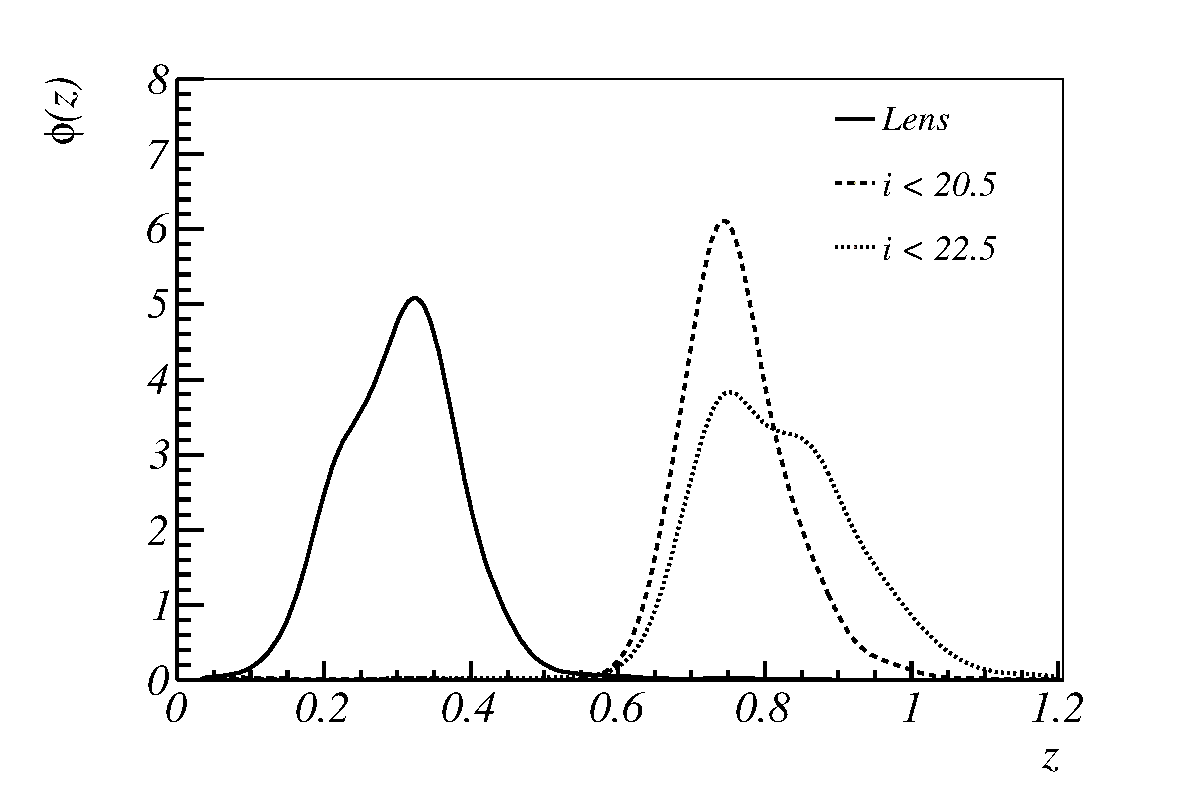
\includegraphics[width=0.85\textwidth]{./figures/TPZ_phis_i.pdf}
\caption{Redshift distributions from the stacking of the TPZ probability distribution functions for the lens and two {\it i}-band sub-samples of the source.}
\label{fig:stacking}
\end{center}
\end{figure}
\newline

Photometric redshifts (photo-z) have been estimated using different techniques. In particular, the fiducial code used in this work employs a machine-learning algorithm (random forests) as implemented by TPZ \cite{2013MNRAS.432.1483C}, which was shown to perform well on SV data \cite{2014MNRAS.445.1482S}. The redshifts of the galaxies are defined according to the mean of the probability density functions given by TPZ ($z_{\rm ph}$). Other methods are also employed to demonstrate that the measured two-point angular cross-correlation are not a feature induced by TPZ.

\subsubsection{Lens sample}
A unique lens sample is defined by the additional photo-z and magnitude cuts:
\begin{itemize}
	\item $0.2 < z_{\rm ph} < 0.4$;
	\item $18.0 < i < 22.5$.
\end{itemize}
These requirements are imposed in order to be compatible with the first redshift bin of the so called `benchmark sample' \cite{2016MNRAS.455.4301C}. Note that the {\scshape mag\_auto} cut along with the previous $i$-band depth cut guarantees uniformity \cite{2016MNRAS.455.4301C}.

\subsubsection{Source sample}
Three source samples are defined, one per band:
\begin{itemize}
	\item R: $0.7 < z_{\rm ph} < 1.0$ and $r<23.0$;
	\item I: $0.7 < z_{\rm ph} < 1.0$ and $i<22.5$;
	\item Z: $0.7 < z_{\rm ph} < 1.0$ and $z<22.0$.
\end{itemize}

Following the same approach we used on the lens, defined over the `benchmark' sample, the {\scshape mag\_auto} cut along with the previously defined depth cuts also guarantee uniformity on the corresponding band. Within each R, I, Z source sample five sub-samples that map the magnitude evolution are defined,
\begin{itemize}
	\item $\rm R_1$: $r<21.0$; $\rm R_2$: $r<21.5$; $\rm R_3$: $r<22.0$; $\rm R_4$: $r<22.5$; $\rm R_5$: $r<23.0$.
	\item $\rm I_1$: $i<20.5$; $\rm I_2$: $i<21.0$; $\rm I_3$: $i<21.5$; $\rm I_4$: $i<22.0$; $\rm I_5$: $i<22.5$.
	\item $\rm Z_1$: $z<20.0$; $\rm Z_2$: $z<20.5$; $\rm Z_3$: $z<21.0$; $\rm Z_4$: $z<21.5$; $\rm Z_5$: $z<22.0$.
\end{itemize}
Here $\rm S_j$ with $\rm j=1,2,3,4,5$ are the sub-samples of sample S with $\rm S\in \{R,I,Z\}$. In \autoref{fig:stacking}, the redshift distributions of the lens and source sample are shown. Note that the sub-samples $\rm R_5, I_5, Z_5$ are equal to $\rm R, I , Z$ respectively.
\newline

The {\it g}-band is not used on this analysis because when the same approach is followed and a uniform sample is defined in that band, the number of galaxies of the lens and source samples decrease dramatically. This increases the shot noise preventing the measurement of number count magnification

\subsection{Detection of the weak-lensing magnification signal}
\label{sec:analysis_sv}
To estimate the cross-correlation functions, the tree-code {\scshape TreeCorr}\footnote{github.com/rmjarvis/TreeCorr} \cite{2004MNRAS.352..338J} and the Landy-Szalay estimator \cite{1993ApJ...412...64L} are used demanding six logarithmic angular bins:
\begin{equation}
\omega_{\rm LS_j}(\theta) = \frac{D_{\rm L}D_{\rm S_j}(\theta)-D_{\rm L}R_{\rm S_j}(\theta)-D_{\rm S_j}R_{\rm L}(\theta)}{R_{\rm L}R_{\rm S_j}(\theta)}+1,
\label{eq:landyszalay}
\end{equation}
where $D_{\rm L}D_{\rm S_j}(\theta)$ is the number of pairs from the lens data sample L and the source data sub-sample $\rm S_j$ separated by an angular distance $\theta$ and $D_{\rm L}R_{\rm S_j}(\theta)$, $D_{\rm S_j}R_{\rm L}(\theta)$, $R_{\rm L}R_{\rm S_j}(\theta)$ are the corresponding values for the lens-random, source-random and random-random combinations normalized by the total number of objects on each sample.
\newline

Catalogs produced with {\scshape Balrog}\footnote{github.com/emhuff/Balrog} \cite{2016MNRAS.457..786S} are used as random sample. See \autoref{sec:balrog} for a detailed description and discussion on this.
\newline

A covariance matrix is computed for each band by jack-knife re-sampling the data taking into account the correlations between the different magnitude cut within each band
\begin{eqnarray}
C_{\rm S}(\omega_{\rm LS_i}(\theta_\eta);\omega_{\rm LS_j}(\theta_\nu)) = \frac{N_{\rm JK}}{N_{\rm JK}-1}\\
\times \sum\limits_k^{N_{\rm JK}}[\omega_{\rm LS_i}^k(\theta_\eta)-\omega_{\rm LS_i}(\theta_\eta)][\omega_{\rm LS_j}^k(\theta_\nu)-\omega_{\rm LS_j}(\theta_\nu)]\nonumber,
\end{eqnarray}
where $\omega^k_{\rm LS_j}$ stands for the cross-correlation of the $k$-th jack-knife re-sample and $\omega_{\rm LS_j}$ is the cross-correlation of the full sample. The $N_{\rm JK}= 120$ jack-knife regions are defined by a $k$-means algorithm \cite{macqueen1967some} using Python's machine learning library {\scshape scikit-learn}\footnote{scikit-learn.org} \cite{scikit-learn}. In order to get $N_{\rm JK}$ regions with equal area, the algorithm is trained on a uniform random sample following the footprint of the data demanding $N_{\rm JK}$ centers. The regions used on the re-sampling are composed by the Voronoi tessellation defined by these centers. These matrices trace the angular covariance as well as the covariances between functions within each band. No covariance between bands is considered, since each band is treated independently on this work. The reduced covariance matrix of the {\itshape i}-band is displayed at \autoref{fig:cov_matrix}. The behaviour is similar for the other bands.
\begin{figure}
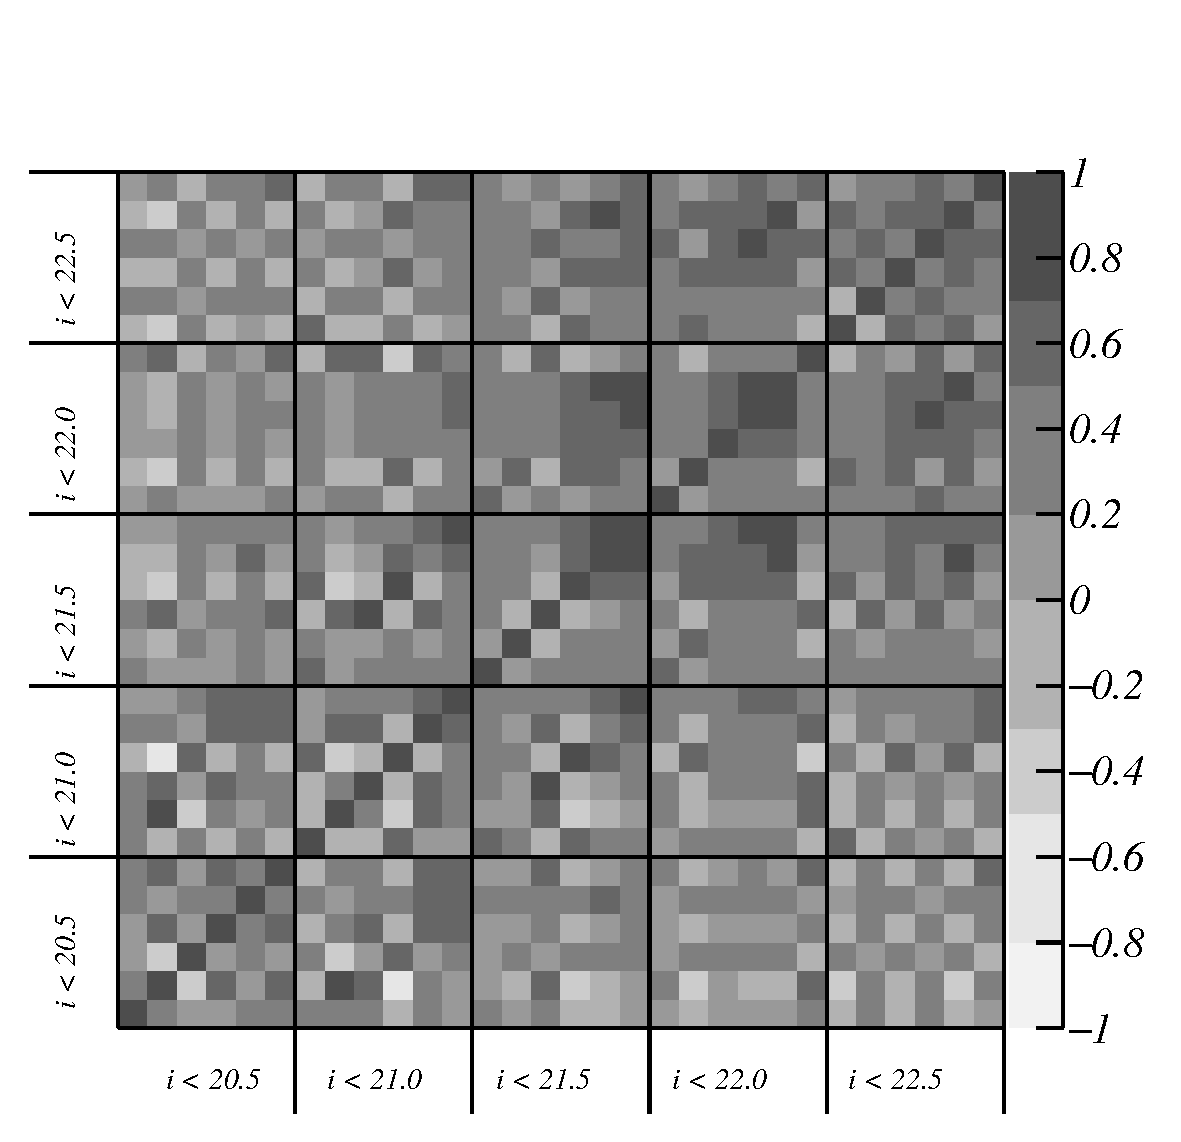
\includegraphics[width=\textwidth,trim={0 0 0 2cm},clip]{./figures/cov_matrix_mag_auto_i.pdf}
\caption{Covariance matrix of the {\it i}-band rescaled by the value of the diagonal ($C_{ij}/\sqrt{C_{ii}C_{jj}}$). Each box is the part of the matrix corresponding to the samples labeled at the axis whereas the bins within each box stand for the angular values of the correlation function.}
\label{fig:cov_matrix}
\end{figure}
\newline

Measured two-point angular cross-correlation functions and $\Lambda$CDM weak lensing theoretical predictions can be found in \autoref{fig:resultsSV_r}, \autoref{fig:resultsSV_i} and \autoref{fig:resultsSV_z}. Measured correlation functions are found to be non-zero, compatible with $\Lambda$CDM and its amplitude evolves with the magnitude cut. The magnitude cuts imposed to guarantee uniform depth make that, for this data, no negative amplitudes are expected.
\begin{sidewaysfigure}
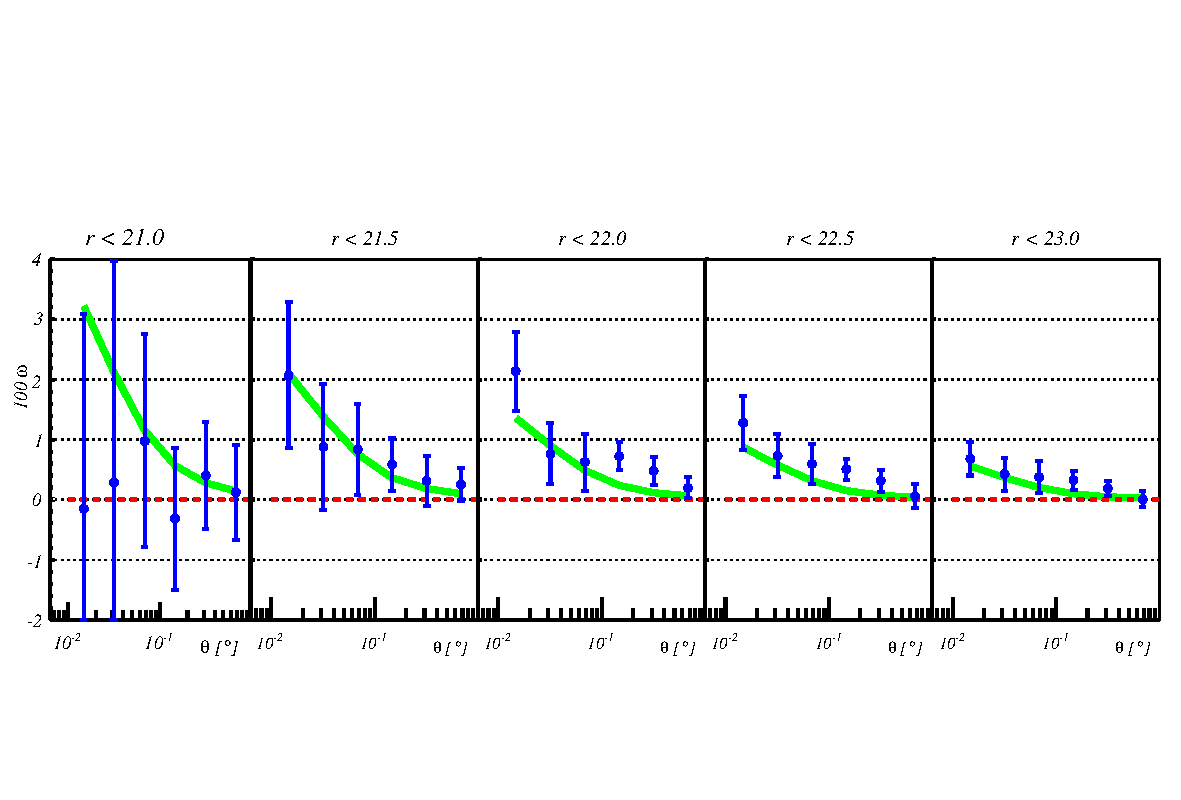
\includegraphics[width=\textwidth,trim={0 2.3cm 0 3.5cm},clip]{./figures/mag_r.pdf}
\label{fig:resultsSV_r}
\caption{Magnification signal for the DES-SV {\it r}-band sample.}
\end{sidewaysfigure}
\begin{sidewaysfigure}
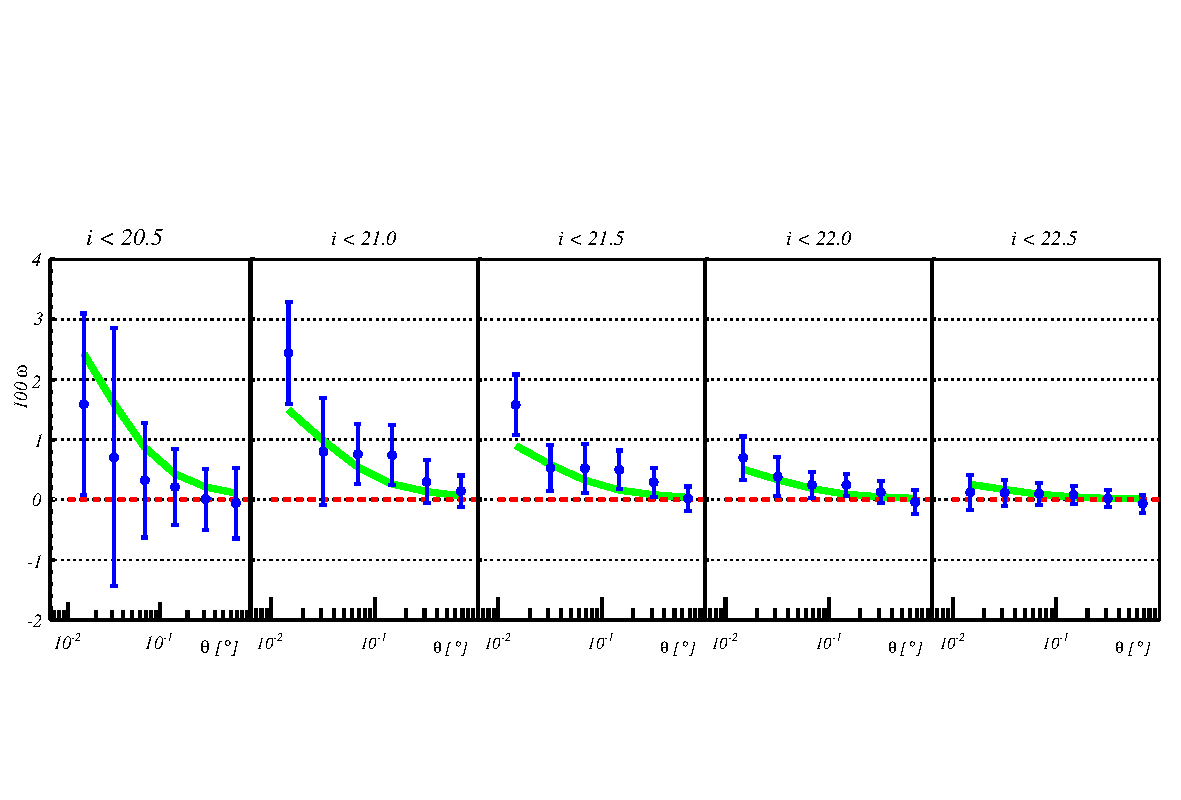
\includegraphics[width=\textwidth,trim={0 2.3cm 0 3.5cm},clip]{./figures/mag_i.pdf}
\label{fig:resultsSV_i}
\caption{Magnification signal for the DES-SV {\it i}-band sample.}
\end{sidewaysfigure}
\begin{sidewaysfigure}
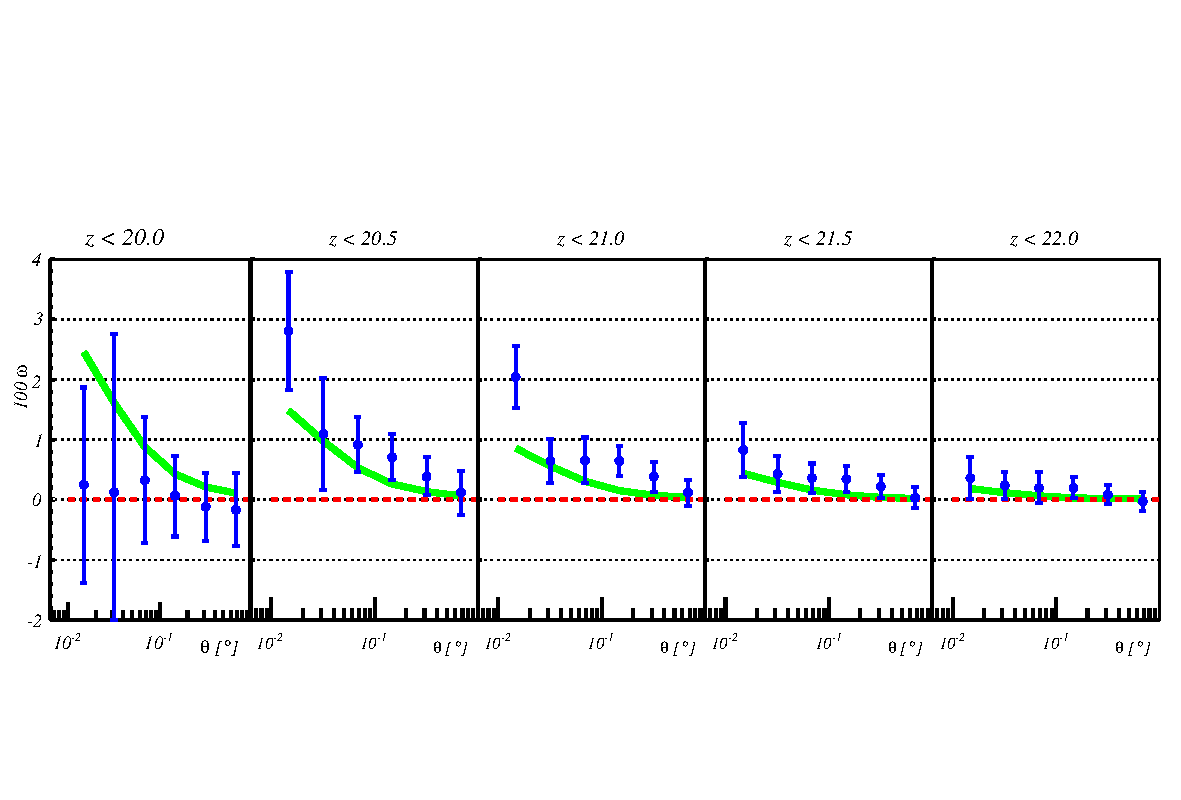
\includegraphics[width=\textwidth,trim={0 2.3cm 0 3.5cm},clip]{./figures/mag_z.pdf}
\label{fig:resultsSV_z}
\caption{Magnification signal for the DES-SV {\it z}-band sample.	}
\end{sidewaysfigure}
\newline

To compare with the expected theory, \autoref{eq:kappa_nc} and \autoref{eq:omega0} and  have been used assuming Planck 2015 \cite{2016A&A...594A..13P} cosmological parameters. The bias of the lens sample has already been measured independently with different techniques: clustering \cite{2016MNRAS.455.4301C}, gg-lensing \cite{2016arXiv160908167P}, shear \cite{2016MNRAS.459.3203C} and CMB-lensing \cite{2016MNRAS.456.3213G}. From these values the most precise, from \cite{2016MNRAS.455.4301C}, is selected ($b_{\rm L}=1.07\pm0.08$) and is assumed to be a constant scale-independent parameter. The number count slope parameter $\alpha_{\rm S}$ is computed by fitting the cumulative number count of the sample S to a Schechter function \cite{1976ApJ...203..297S} on the range of interest
\begin{equation}
N_\mu(m) = A\left[10^{0.4(m-m_*)}\right]^\beta\times\exp\left[-10^{0.4(m-m*)}\right],
\label{eq:sch}
\end{equation}
where $A,m_*,\beta$ are the free parameters of the fit. Then $\alpha_{\rm S}(m)-1$ is computed by applying \autoref{eq:alpha}, where $m_{\rm j}$ is the magnitude limit of the $\rm S_j$ sub-sample on the considered band. In \autoref{fig:alphai} the fit and the number count slope parameter for the I sample are shown.
\begin{figure}
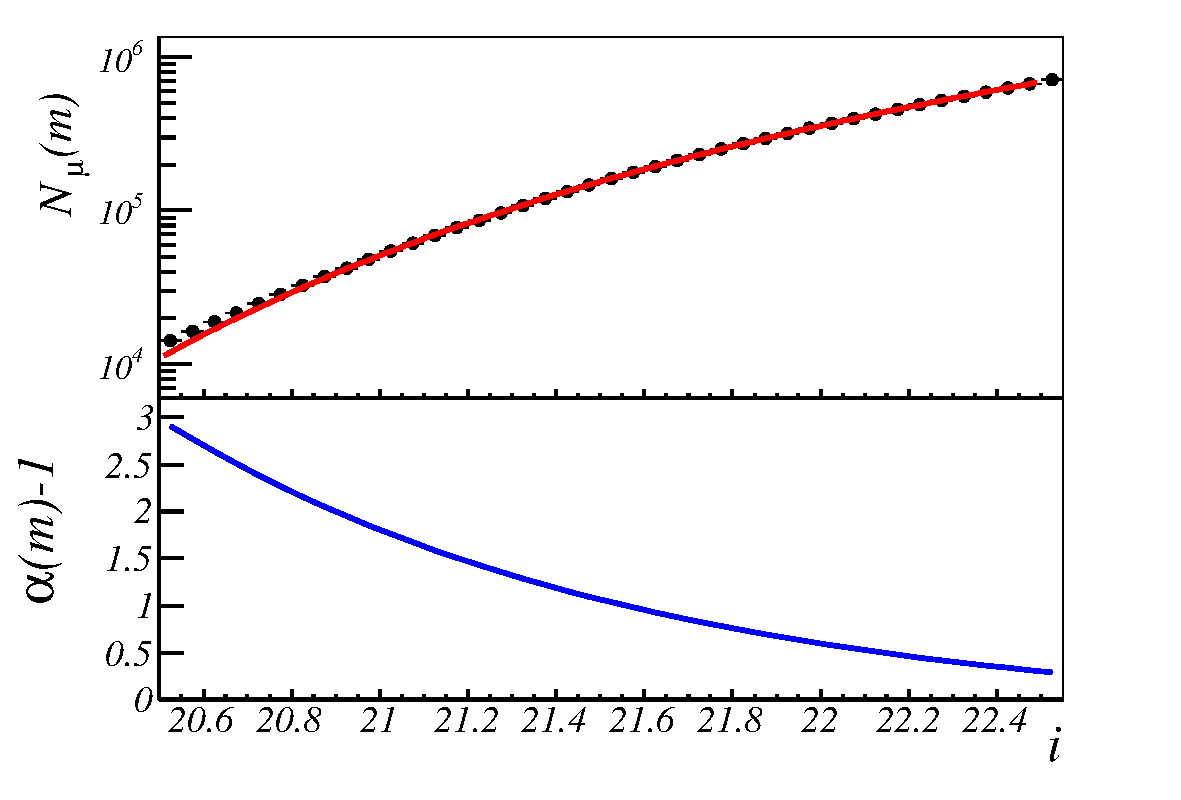
\includegraphics[width=0.85\textwidth]{./figures/alphai.pdf}
\caption{Top panel: Dots are the measured {\it i}-band cumulative number count as a function of the {\it i}-band magnitude. Red solid line is the fit using a Schechter function (see text). Bottom panel: number count slope $\alpha-1$ measured from the fitted Schechter function of the top panel.}
\label{fig:alphai}
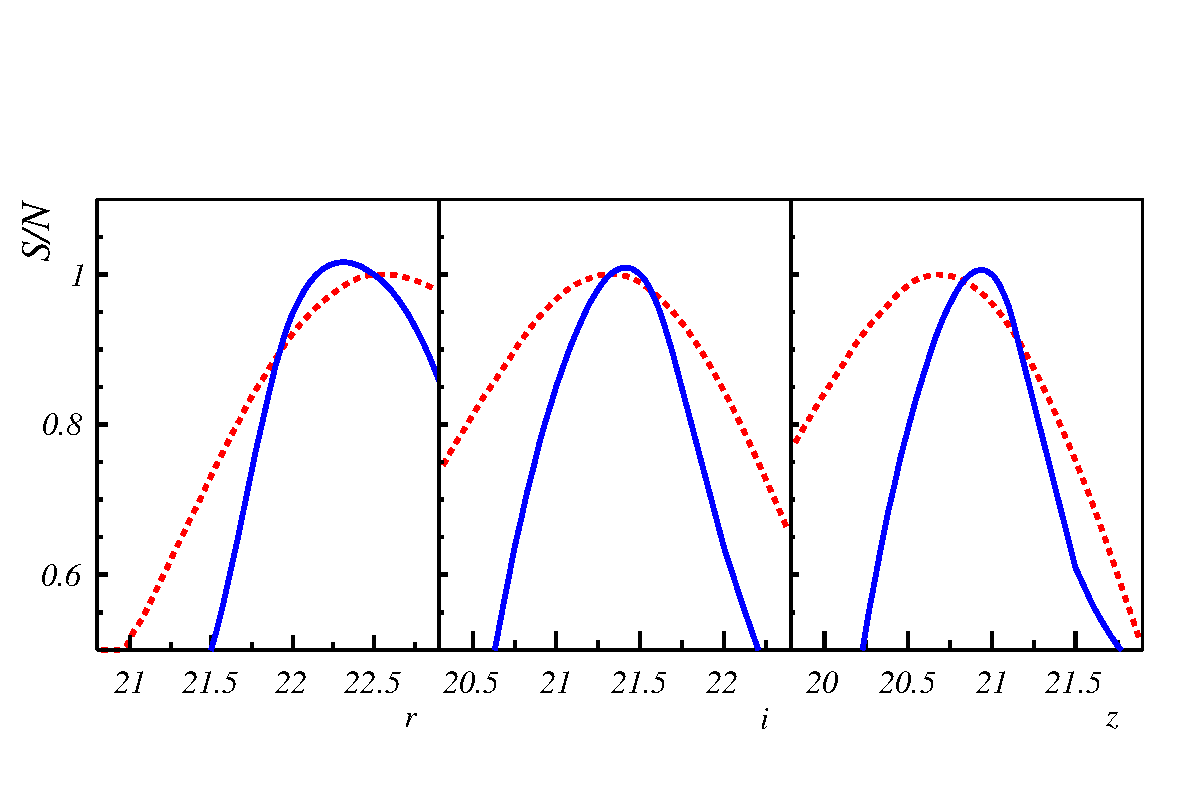
\includegraphics[width=0.85\textwidth,trim={0 1.0cm 0 2.5cm},clip]{./figures/predicted_sig.pdf}
\caption{Red dashed line: expected signal-to-noise ratio computed with \autoref{eq:sn}. Blue solid line is the measured significance of the data. Both curves are normalized to their respective maximum.}
\label{fig:significance}
\end{figure}
\begin{table}
\begin{center}\begin{tabular}{ c | c | c c }
 Weight& Sample & $\log_{10}\mathcal{B}$ & $\chi^2/ndof$  \\
\hline
 & R & 3.9 & 21.6/30\\
 No& I & 3.4 & 23.9/30\\
 & Z & 3.4 & 36.8/30\\
\hline
 & $r<23.0$ & 3.2 & 3.2/6\\
 Yes& $i < 22.5$ & 2.1&2.1/6\\
 & $z<22.0$ & 2.3&2.3/6\\
\end{tabular}\end{center}
\caption{Significance of the detection of a magnification signal. Results are shown for the combination of the five subsamples within each band as well as for the faintest sample with weighting.}
\label{tab:significance}
\end{table}
\newline

A goodness of fit test of the measured two-point angular cross-correlation function respect to the theoretical predictions for each band is performed:
\begin{eqnarray}
&\chi^2_{\rm Planck} =\sum\limits_{\eta\nu ij}[\tilde \omega_{\rm LS_i}(\theta_\eta)-\omega_{\rm LS_i}(\theta_\eta)]\\
&C^{-1}(\omega_{\rm LS_i}(\theta_\eta);\omega_{\rm LS_j}(\theta_\nu))[\tilde \omega_{\rm LS_j}(\theta_\nu)-\omega_{\rm LS_j}(\theta_\nu)],
\end{eqnarray}
where $\tilde\omega,\omega$ are the measured and theoretical cross-correlation functions respectively. Goodness of fit tests are also made testing the hypothesis of absence of magnification:
\begin{eqnarray}
&\chi^2_{\rm zero}=\\
&\sum\limits_{\eta\nu ij}\tilde\omega_{\rm LS_i}(\theta_\eta)C^{-1}(\omega_{\rm LS_i}(\theta_\eta);\omega_{\rm LS_j}(\theta_\nu))\tilde\omega_{\rm LS_j}(\theta_\nu)\nonumber.
\end{eqnarray}
The $\chi^2$ values can be seen in \autoref{tab:significance} showing good agreement with the theoretical predictions described in \autoref{ch:theory}. To test which hypothesis is favored, the Bayes factor is used:
\begin{equation}
\mathcal{B} = \frac{P(M|\Theta)}{P(Z|\Theta)} = \frac{P(\Theta |M)}{P(\Theta|Z)}\frac{P(M)}{P(Z)},
\end{equation}
where 
\begin{equation}
P(M|\Theta) = e^{-\chi^2_{\rm Planck}/2}
\end{equation}
and
\begin{equation}
P(Z|\Theta) = e^{-\chi^2_{\rm zero}/2}.
\end{equation}
The assumed prior sets detection and non-detection of magnification to be equally probable: $P(M) = P(Z)$. Bayes factors are computed for each function individually as well as for each band using the full covariance.
\newline

The significance for each individual correlation function has a strong dependence on the considered magnitude limit of the sub-sample. At the bright cuts, shot-noise prevents the identification of a non-zero magnification signal. At the faint end, although the sub-samples are much more populated, the strength of the magnification signal is compatible with zero. This behaviour has been compared with the predictions (see \autoref{sec:method}). Predicted and measured values are plotted together in \autoref{fig:significance}. It can be seen that the prediction of the location of the maximum signal-to-noise can only be used as a first approach.
\newline

To compute the significance of the detection for each band, the full covariance is used. One covariance matrix (see \autoref{fig:cov_matrix} for the {\itshape i}-band matrix) per each band is computed taking into account the correlations between each magnitude cut. The logarithm of the Bayes factor can be found in \autoref{tab:significance}, being all above 2, allowing to claim that magnification has been detected \cite{10.2307/2291091}.
\newline
 
 A usual approach to enhance the signal-to-noise ratio, is to define a unique source sample and weight each source galaxy with its corresponding $\alpha_S(m)-1$ value \cite{2003A&A...403..817M} and compute the two-point angular cross-correlation function. This weighting procedure is used at the samples $r < 23.0$, $i < 22.5$ and $z < 22.0$. These correlation functions can be seen in \autoref{fig:reweight} with a comparison with the theoretical prediction and the correlation functions of the same sample computed without weighting. Significances of these measurement can be found in \autoref{tab:significance} with a marginal difference respect to the one computed without weighting using the five subsamples.
\begin{figure}
\begin{center}
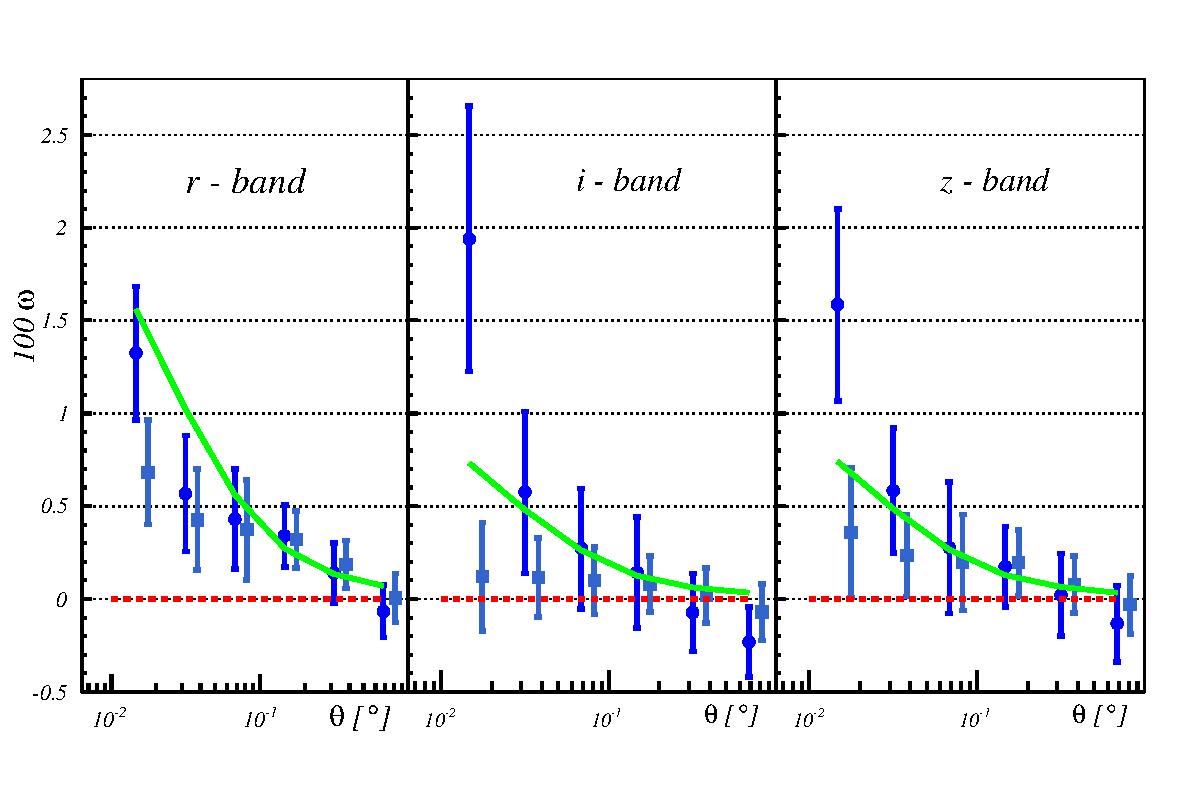
\includegraphics[width=0.85\textwidth]{./figures/weighted_w.pdf}
\caption{Measured two-point angular cross-correlation functions for the samples $r<23.0$, $i < 22.5$ and $z < 22.0$ left to right respectively. Dots use the optimal weighting \cite{0004-637X-633-2-589}, where each galaxy is weighted by its corresponding $\alpha_S(m)-1$ value, whereas squares are not weighted. Green line is the theoretical prediction. Red dashed line is an eye-guide for zero.}
\label{fig:reweight}
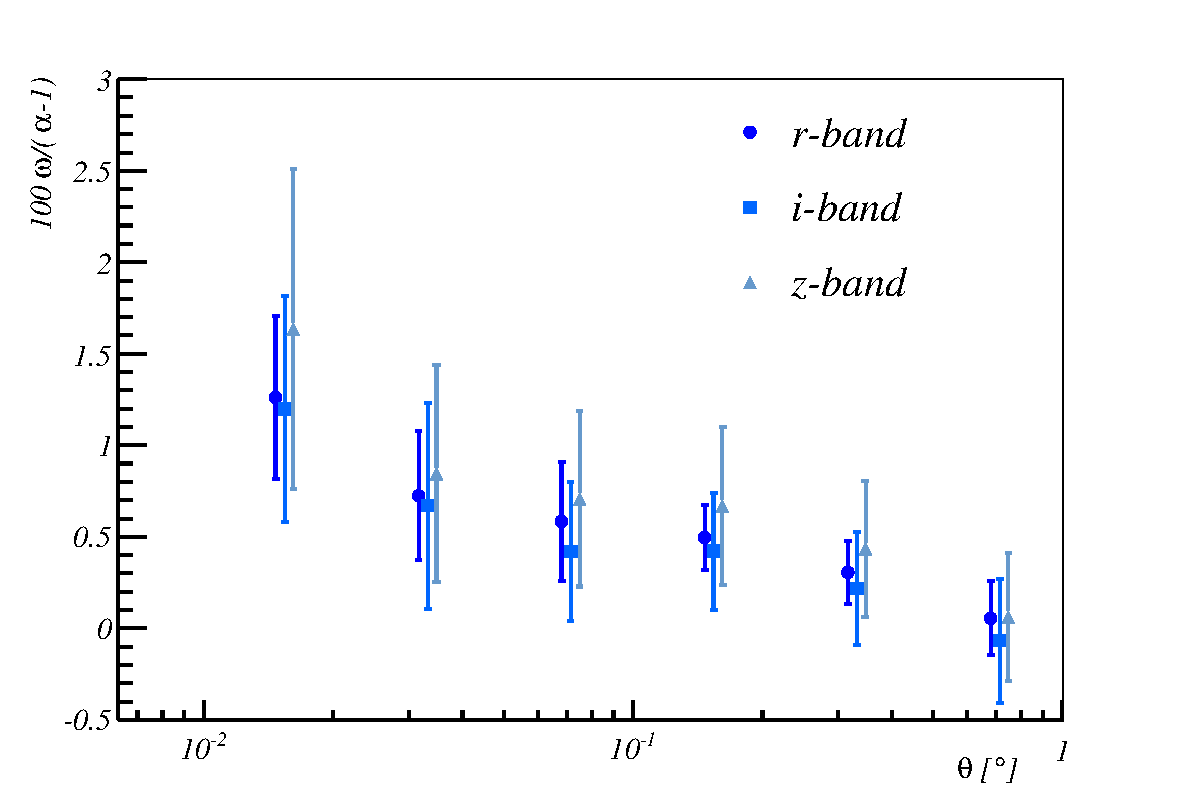
\includegraphics[width=0.85\textwidth]{./figures/acromatic_short.pdf}
\caption{Example of the achromaticity of the measured signal. Here are shown the measured two-point angular cross-correlation functions for $r<22.5$, $i<22.0$ and $z<21.5$ divided by their corresponding $\alpha-1$.}
\label{fig:achrom}
\end{center}
\end{figure}
\newline
 
 Finally, in order to test that the signal is achromatic, the measured two-point angular cross-correlation functions for each band, normalized by its $\alpha_S(m)-1$ are compared. All cross-correlation functions fluctuate within $1\sigma$ errors (see \autoref{fig:achrom} for an example) demonstrating that the measured convergence field does not depend on the considered band.

\subsection{Systematic error analysis}
\label{sec:sys}
Here, the impact of potential sources of systematic errors on the measured two-point angular cross-correlation function is investigated and how they are taken into account in the measurement is described.

\subsubsection{Number count slope $\alpha$}
    
\begin{figure}
\begin{center}
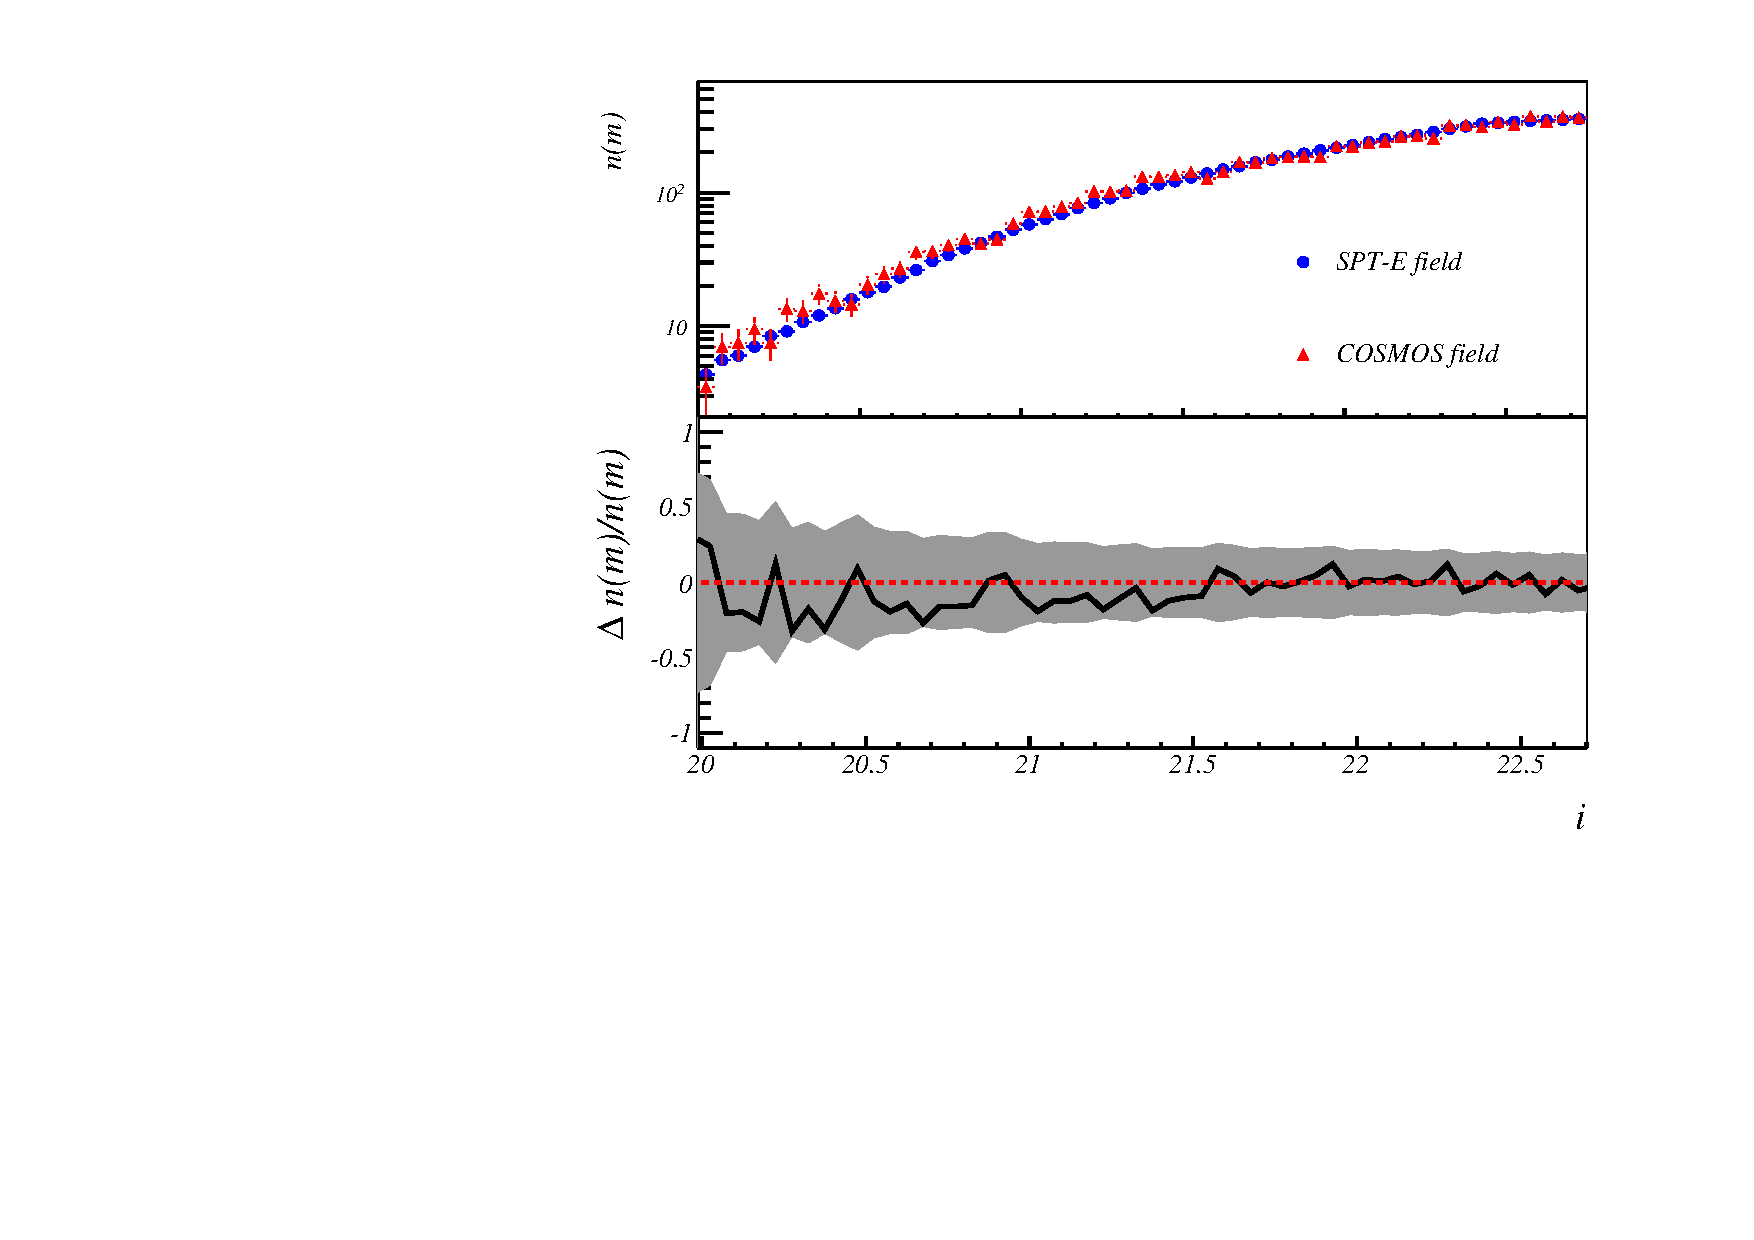
\includegraphics[width=0.85\textwidth]{./figures/SPTE_SNe.pdf}
\caption{Upper panel: Comparison of the magnitude distribution for the SPT-E and the COSMOS fields. Both histograms are normalized by their respective area. Lower panel: Relative difference between the magnitude distribution of the COSMOS and the SPT-E fields. The shaded region shows the $1\sigma$ confidence interval computed from shot-noise.}
\label{fig:ndmSN}
	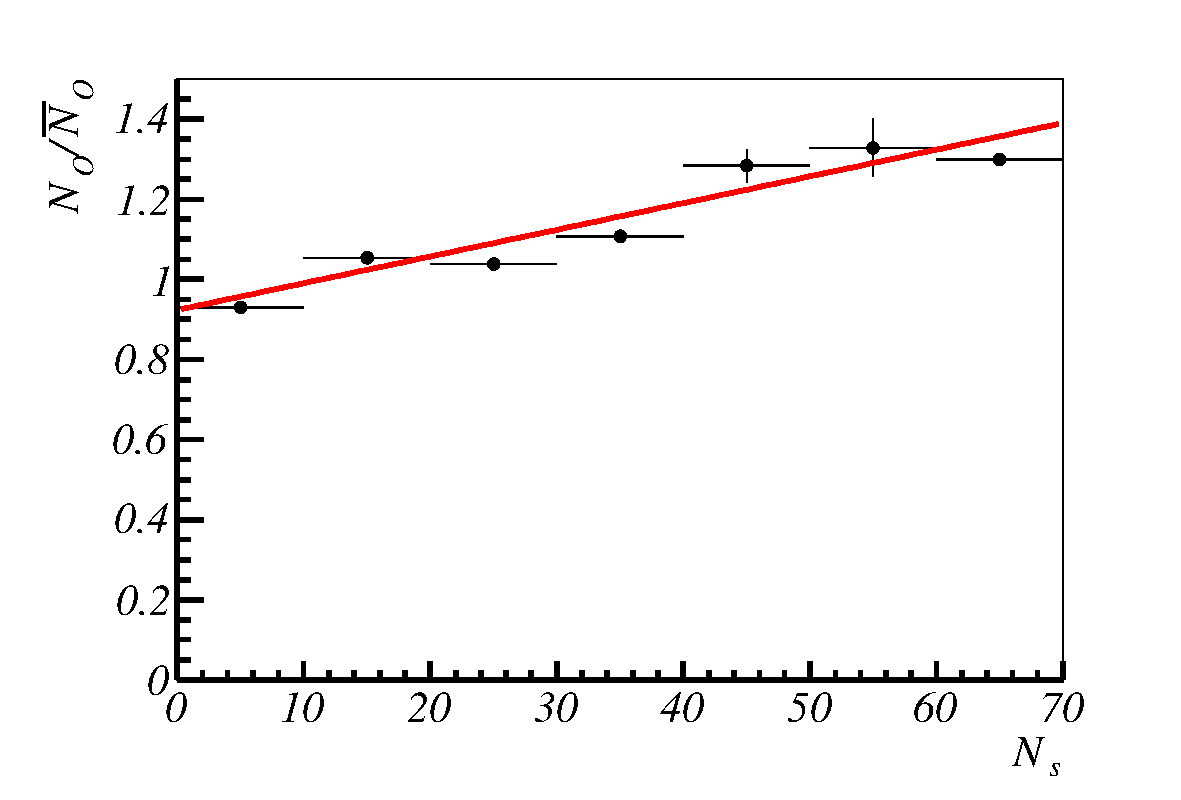
\includegraphics[width=0.85\textwidth]{./figures/purity_lens.pdf}
    \caption{Determination of the purity of the lens sample. For each $N_{\rm nside}=512$ {\scshape HEALPix}-pixel, the number of objects classified as galaxies divided by the average number of galaxies per pixel is plotted as a function of the  number of objects classified as stars. Black dots are the measured data. Red line is the linear fit to the data. The intercept of the line with the Y-axis is the estimated purity of the sample.}
    \label{fig:purity}
    \end{center}
\end{figure}
	When comparing the measured two point angular cross-correlation functions with the theoretical prediction via \autoref{eq:kappa_nc} for a given set of cosmological parameters, $\alpha(m)$ is determined by fitting the cumulative number count distribution to \autoref{eq:sch} and then using \autoref{eq:alpha}. To compute the possible impact of the uncertainty of this fit on the comparison with theory, a marginalisation over all the parameters of fit ($A,m_*,\beta$) is made.
\newline
	
Parameters are randomly sampled with a Gaussian distribution centerd on the value given by the fit to the cumulative number count and with a standard deviation equal to the $1\sigma$ errors of the fit. The value of $\alpha$ is recalculated with these randomly sampled parameters. The impact of the dispersion of the $\alpha$ values obtained is negligible compared to the size of the jackknife errors, so they are not taken into account.
\newline

In addition to the parameter determination, a possible non-completeness on the SPT-E field can modify the magnitude distribution altering the cumulative number count slope parameter \cite{2016MNRAS.455.3943H}. To estimate the possible impact of non-completeness, the measured magnitude distributions of the SPT-E field are compared with those of deeper fields measured by DES, such as the COSMOS field. Both distributions are found to be equal at the range of magnitudes considered on this analysis (see \autoref{fig:ndmSN} for an example in the $i$-band).

\subsubsection{Object obscuration}

Chang \cite{0004-637X-801-2-73} studied whether moderately bright objects in crowded environments produce a decrease in the detection probability of nearby fainter objects at scales $\theta\lesssim10\ $arcsec. However, such scales are well below those considered in this analysis ($\theta>36$ arcsec) and therefore this effect is ignored.

\subsubsection{Stellar contamination}
    
	For a given choice of star-galaxy classifier, there will be a number of stars misclassified as galaxies, so the observed two-point angular cross-correlation function $\omega_O(\theta)$ must be corrected by the presence of any fake signal induced by stars (see \cref{sec:starscorrection}):
	\begin{equation}
	\omega_{\rm LS_j} = \frac{\omega_{\rm O}(\theta)-\lambda_{\rm L}\omega_{\rm *S_j}(\theta)-\lambda_{\rm S_j}\omega_{\rm L*}(\theta)}{1-\lambda_{\rm L}-\lambda_{\rm S_j}},
	\label{eq:starcorrection}
	\end{equation}
	where $\omega_{\rm LS_j}$ is the corrected galaxy cross-correlation function, $\omega_{\rm L*}$ is the cross-correlation function of the true galaxy lenses with the stars misclassified as galaxies in the source sample, $\omega_{\rm *S_j}$ is the cross correlation of the stars misclassified as galaxies in the lenses with the true source galaxies and $\lambda_{\rm L},\lambda_{\rm S_j}$ are the fraction of stars in the lens and in the source samples respectively.
	Assuming that the misclassification of stars is spatially random and is a representative sample of the spatial distribution of the population classified as stars and that the fraction of misclassified stars is small, the functions $\omega_{\rm L*},\omega_{\rm *S_j}$ are estimated from the cross-correlation of the galaxy population and the stellar population in the corresponding redshift bin.
    \begin{sidewaysfigure}
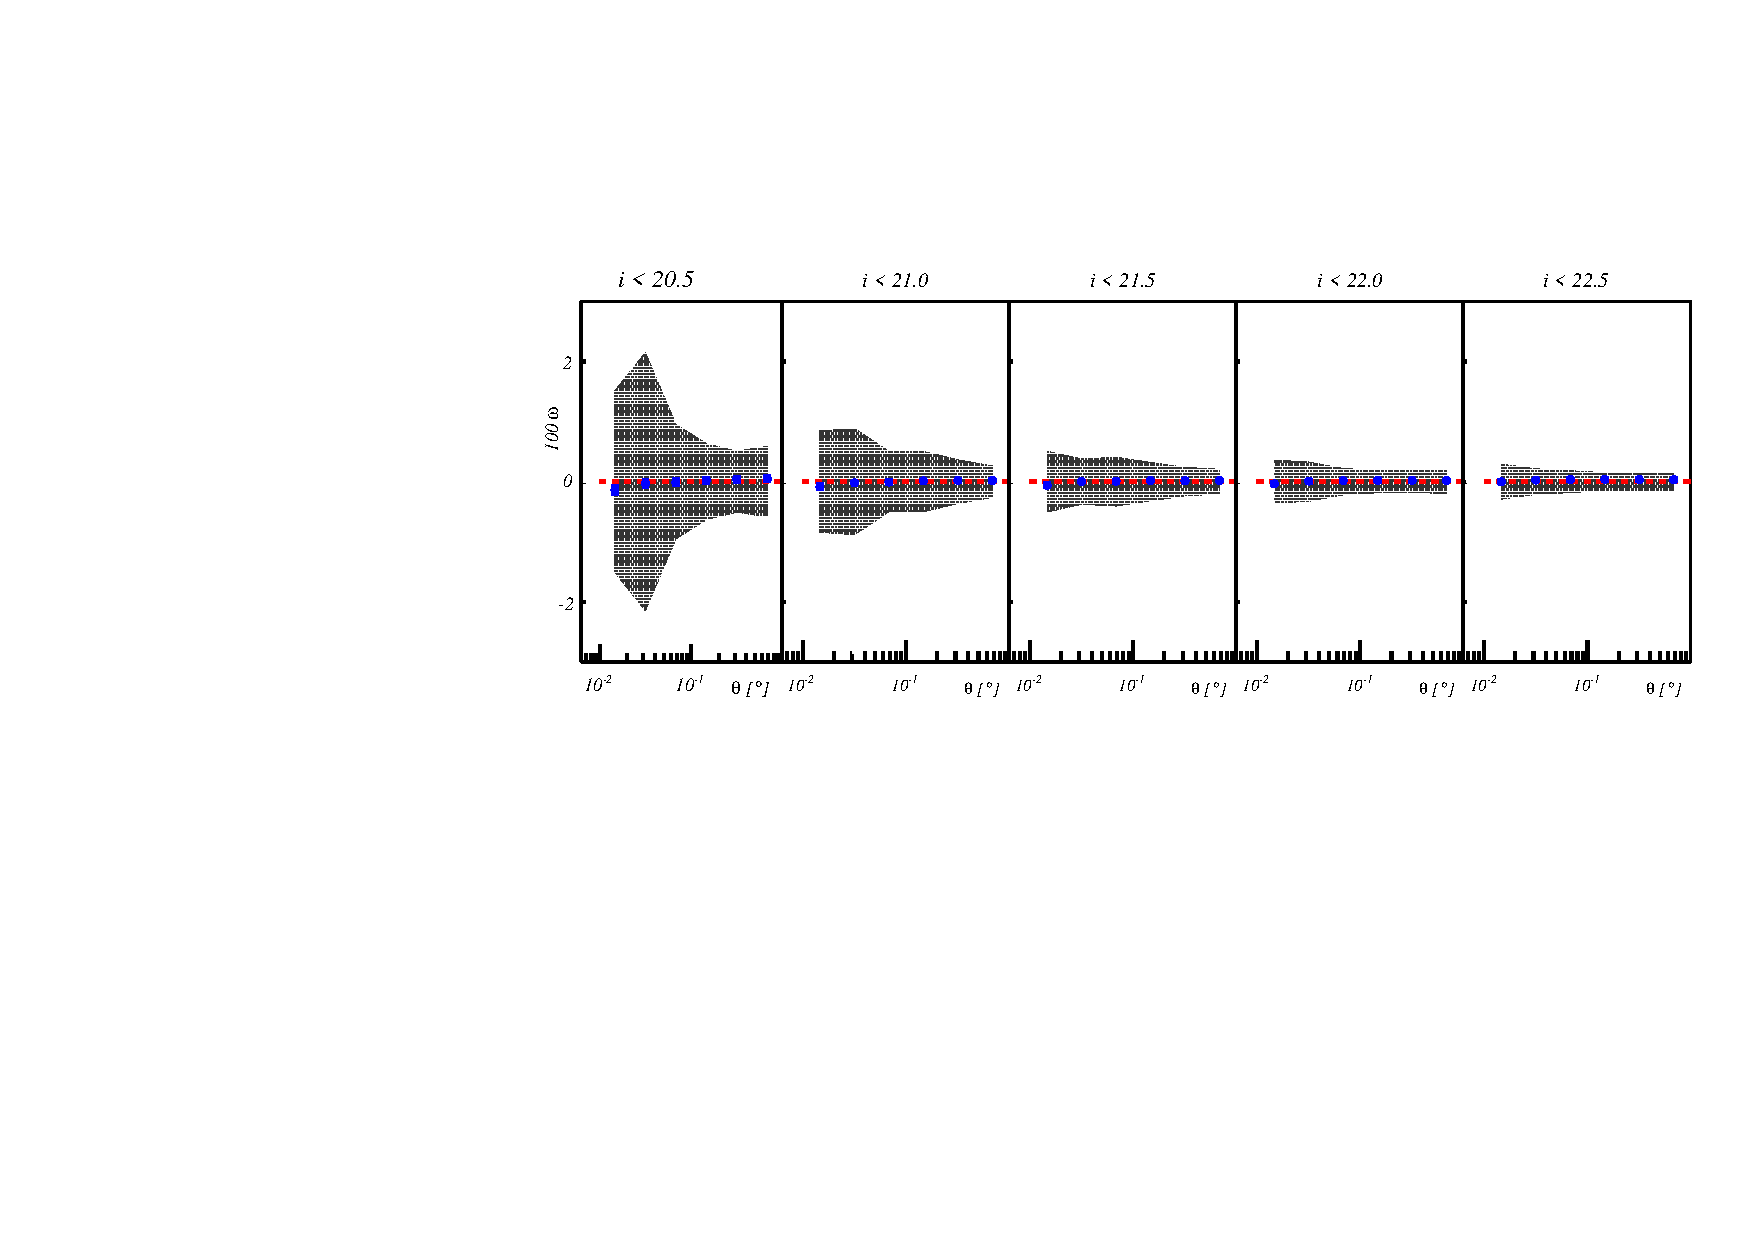
\includegraphics[width=\textwidth,trim={0 2.3cm 0 3.5cm},clip]{./figures/mag_istars.pdf}
\caption{Correction by stellar contamination on the $i<21.5$ sample. Blue dots are the correction and shaded area is the $1\sigma$ confidence interval of the measured cross-correlations of the magnification signal. Red dashed line is and eye-guide for zero.}
\label{fig:correction}
\end{sidewaysfigure}
\newline
 
	Following a similar approach to \cite{2012MNRAS.424..564R}, if the latter is true and the misclassified stars trace the global population of stars, for a given patch of the sky the number of objects classified as galaxies $N_{\rm O}$ must be the average number of true galaxies $\bar N_{\rm g}$ plus a quantity proportional to the number of stars on that given pixel,
	\begin{equation}
	N_{\rm O} = \bar N_{\rm g}+\tilde\gamma N_{\rm s}.
	\end{equation}
	Dividing by the average number of objects marked as galaxies $\bar N_{\rm O}$,
	\begin{equation}
	\frac{N_{\rm O}}{\bar N_{\rm O}} = p+\gamma N_{\rm s},
	\label{eq:purity}
	\end{equation}
	where $p=\bar N_{\rm g}/\bar N_{\rm O}$ is the purity of the sample, that is, $\lambda = 1-p$.
	\newline
	
	In order to estimate the purity of the galaxy sample with this method, an $N_{\rm side}=512$ {\scshape HEALPix} pixelation is made and for each pixel $N_{\rm O}/\bar N_{\rm O}$ and $N_{\rm s}$ is computed. Then, a fit to \autoref{eq:purity} is made determining a purity of 94 per cent for the lens sample and about 98 per cent for the source sample depending on the considered band (see \autoref{fig:purity} for an example). With this purity, the correction due to stellar contamination given by \autoref{eq:starcorrection} is found to be one order of magnitude smaller than the statistical errors (see \autoref{fig:correction} for the $i$-band correction), so stellar contamination is not taken into account in the analysis. Nevertheless, on future analysis with more galaxies and area this may be important. Note that the objects labeled as stars by our star-galaxy classifier would be a combination of stars and galaxies thus these calculations are an upper bound to stellar contamination.

	\subsubsection{Survey observing conditions}
    \label{sec:balrog}
    Observing conditions are not constant during the survey, leading to spatial dependencies across the DES-SV footprint \cite{2015arXiv150705647L} that may affect the observed cross-correlation function, such as seeing variations, air-mass, sky-brightness or exposure time \cite{2015MNRAS.454.3121M}. To trace these spatial variations, the catalog produced by the Monte Carlo sampling code {\scshape Balrog} has been used as random sample \cite{2016MNRAS.457..786S}. It is important to remark that {\scshape Balrog} catalogs are produced with the same pipeline as DES-SV data, allowing one to trace subtle effects such as patchiness on the zeropoints, deblending and possible magnitude errors due to a wrong sky subtraction close to bright objects.
    \newline
    
    The {\scshape Balrog} catalogs are DES-like catalogs, where
no intrinsic magnification signal has been included. The {\scshape Balrog} software generates images of fake objects, all with zero convergence $\kappa$, that are embedded into the DES-SV coadd images
(convolving the objects with the measured point spread function, and applying the measured photometric calibration). Then {\scshape SExtractor} was run on them, using the same DES Data Management configuration parameters used for the image processing. The positions for the simulated objects were generated randomly over the celestial sphere, meaning that these positions are intrinsically unclustered. Hence, the detected {\scshape Balrog} objects amount to a set of random points, which sample the survey detection probability. For a full description and an application to the same measurement as in \cite{2016MNRAS.455.4301C} see \cite{2016MNRAS.457..786S}. This is the first time that this extensive simulation is used to correct for systematics. The same cuts and masking of the data sample (\autoref{sec:data_sample_SV}) are also applied to the the {\scshape Balrog} sample. A re-weighting following a nearest-neighbours approach was applied to {\scshape Balrog} objects in order to follow the same magnitude distribution of the DES-SV data on both lens and sources.
    \newline
    
     The use of Monte Carlo sampling methods provides a new approach to mitigate systematic effects complementary to methods that cross-correlate the galaxy-positions with the maps of the survey observing conditions \cite{2012MNRAS.424..564R,2012ApJ...761...14H,2015MNRAS.454.3121M} or involve masking the regions of the sky with worst values of the observing conditions \cite{2016MNRAS.455.4301C}. The amount of sky to be masked in order to mitigate the systematic effects on the correlation functions, is freely decided based on the impact on the correlation function, which may lead to a biassed measurement. On the other hand, the approach involving cross-correlations may lead to an overcorrection effect since the different maps of the observing conditions are, in general, correlated in a complicated manner \cite{2016MNRAS.456.2095E}. This new Monte Carlo technique to sample the selection function of the survey given by {\scshape Balrog}, has the advantage that takes into account the correlation of the different observing conditions maps as well as provides an objective criteria to mitigate systematic errors on the correlation function for a given sample, avoiding biassed measurements. In addition, the use of {\scshape Balrog} has the potential to allow us in the future to exploit the full depth of the survey \cite{2016MNRAS.457..786S}.
\newline

{\scshape Balrog} allows to explore how the {\it real} properties of the galaxies are mapped into the observed ones. One might think that it may be translated from observed to real quantities. This is not possible since that although the $real\rightarrow observed$ map is one-to-one, meanwhile the $observed\rightarrow real$ is not.
\newline

Although the use of {\scshape Balrog} is a ground-breaking technique on the mitigation of systematic errors, its limitation must be taken into account. The simulated catalogs are as good as the input catalogs are an accurate representation of the reality. Thus, if an specific population of galaxies is not on the input, it will not be taken into account. DES-SV {\scshape Balrog} catalogs are based on the {\scshape COSMOS} survey\footnote{cosmos.astro.caltech.edu}, that is based on images from the Hubble Telescope that are deeper than the DES survey. Thus, the overall quality of the input catalog is better than DES. Thus this should not be a limitation on this analysis.

\subsubsection{Dust extinction}
\label{sec:dustext}

\begin{sidewaysfigure}
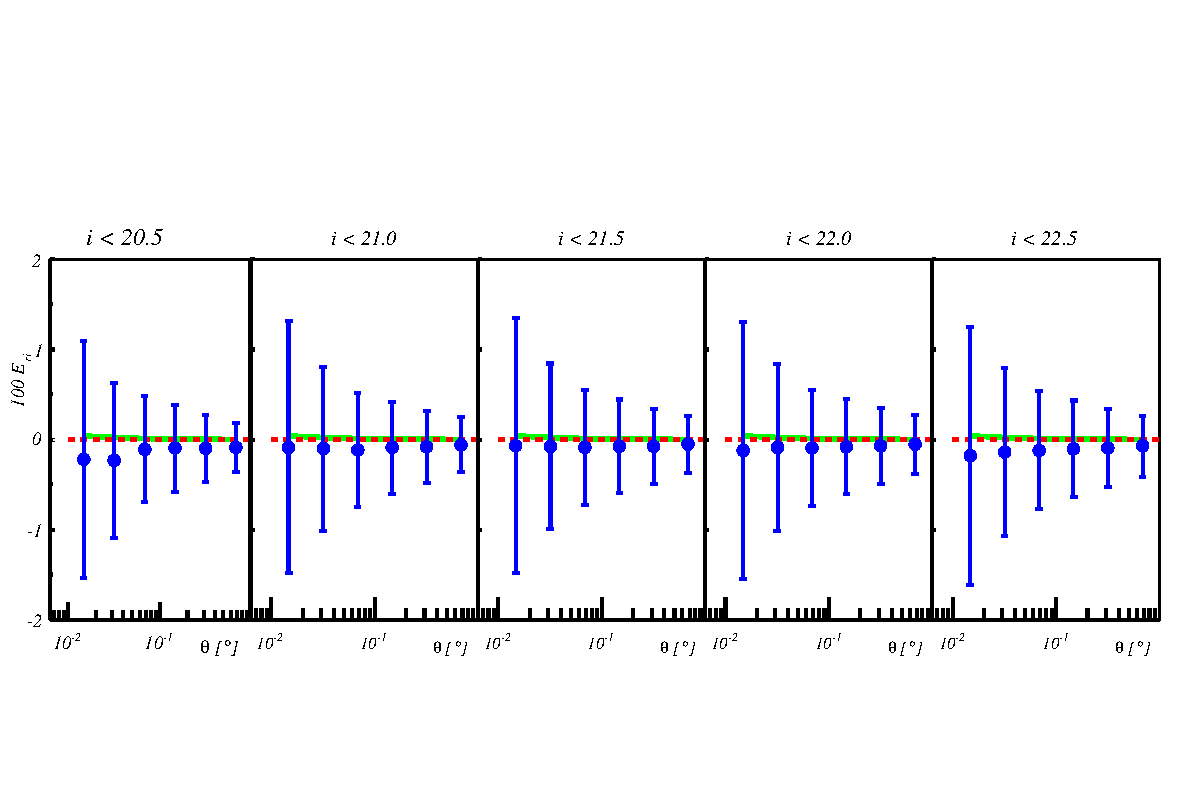
\includegraphics[width=\textwidth,trim={0 2.3cm 0 3.5cm},clip]{./figures/mag_i_ri.pdf}
\caption{Blue dots: color-density cross-correlation functions measured on SV data for the {\it r} and {\it i} bands (sample $i<21.5$). Green solid line is the expected value from \autoref{eq:colorexcess}. Red dashed line is an eye-guide for zero.}
\label{fig:colorexcess}
\end{sidewaysfigure}

\begin{sidewaysfigure}
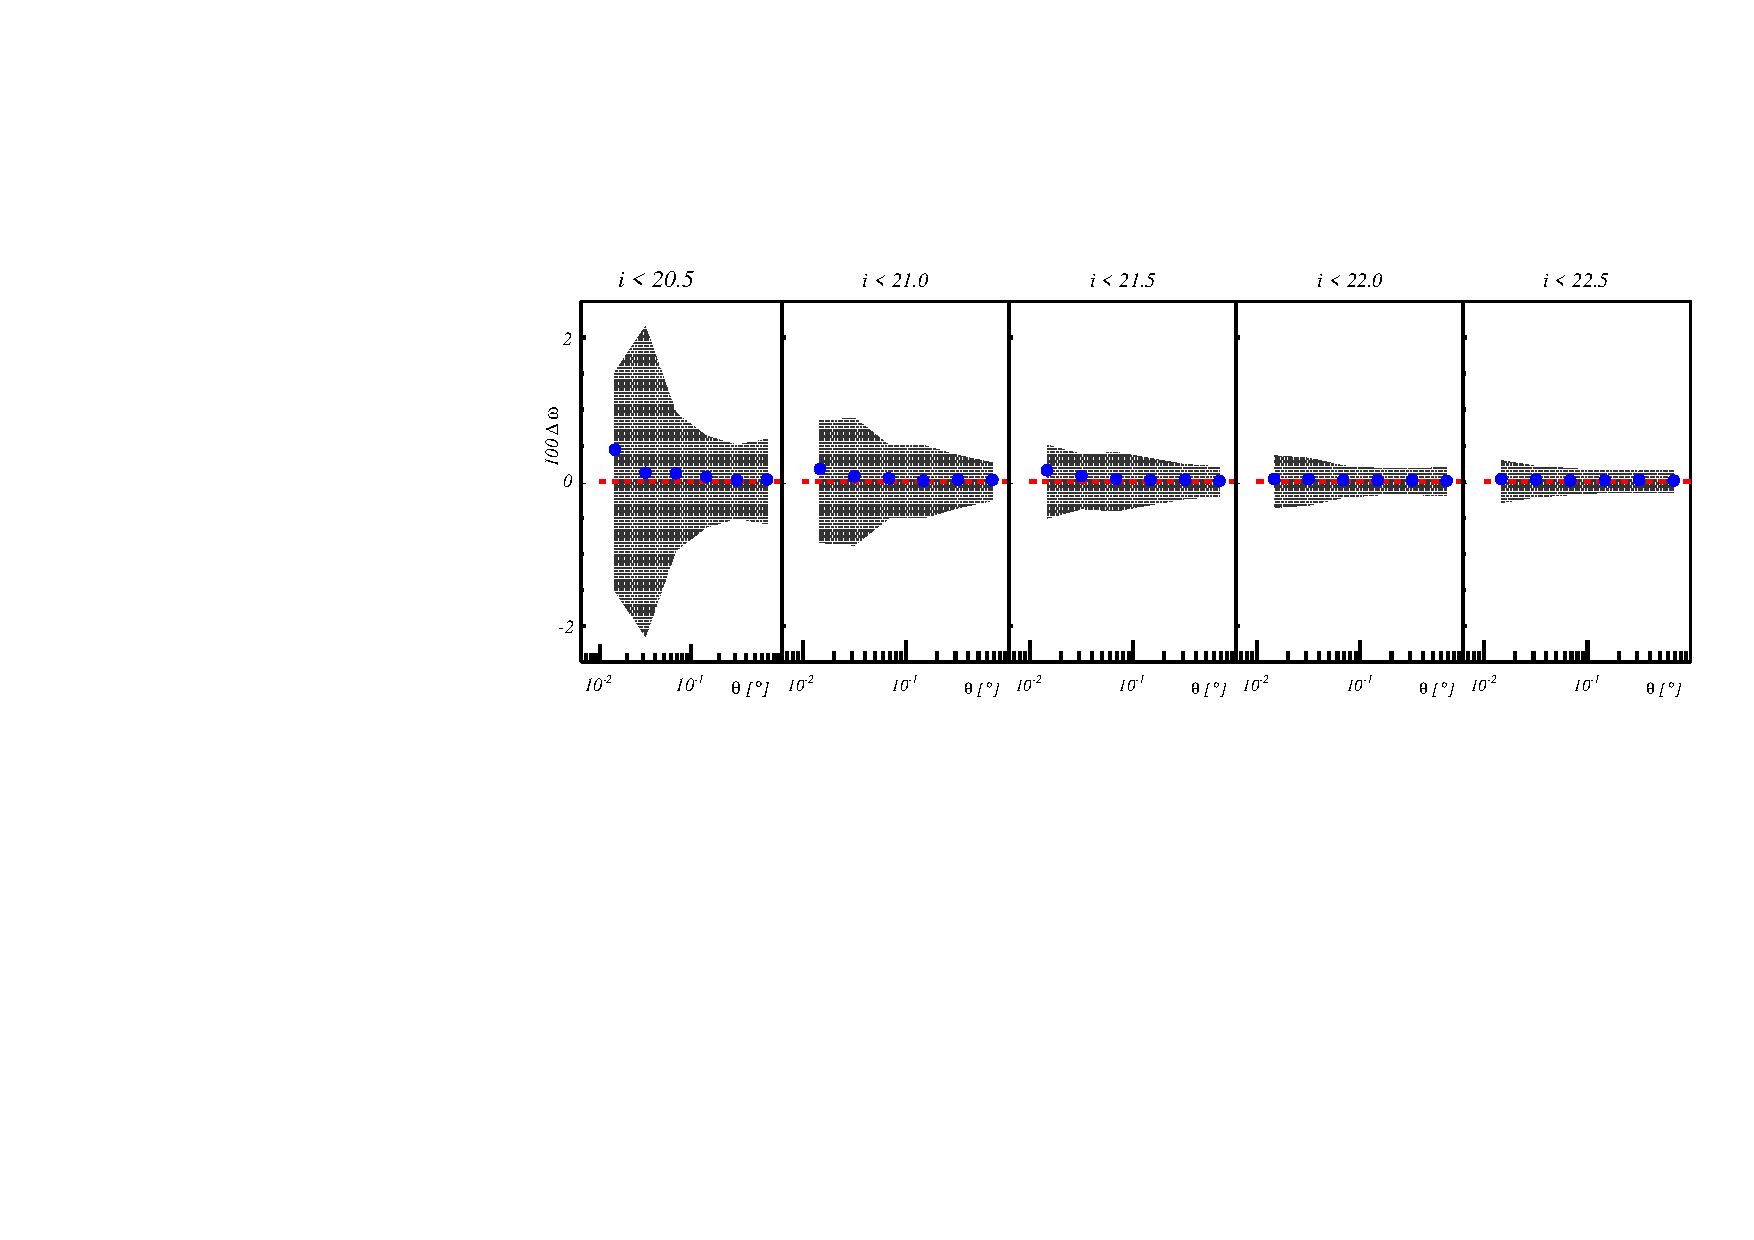
\includegraphics[width=\textwidth,trim={0 2.3cm 0 3.5cm},clip]{./figures/mag_idust.pdf}
\caption{Impact of dust on the number count from MICE (sample $I$). Shade is the $1\sigma$ confidence interval. Blue dots are the number count differences between the case with and the case without the simulated dust profile. Red dashed line is an eye-guide for zero.}
\label{fig:micedust}
\end{sidewaysfigure}
The possible presence of dust in the lenses may modify the observed magnitude in addition to the magnitude shift due to magnification \cite{2010MNRAS.405.1025M}. The change in magnitude ($\delta m$) on the $p$-band may be written as
\begin{equation}
\delta m_p = -2.5\log\mu+\frac{2.5}{\ln10}\tau_p,
\end{equation}
where  $\mu\simeq1+2\kappa$ is the change in magnitude due to magnification and $\tau_k$ is the optical depth due to dust extinction. Whereas magnification is achromatic, dust extinction induces a band-dependent magnitude change. Taking this into account, the color-excess for bands $p,q$\footnote{In this section $p,q$ stand for a generic index label while $V$ stands for the $V$ band of the $UBV$ system.} is defined as
\begin{equation}
E_{pq} = \delta m_p-\delta m_q=1.08[\tau_p-\tau_q].
\end{equation}
Define the color-density cross-correlation as \cite{2010MNRAS.405.1025M}
\begin{equation}
\langle \delta_{\rm g}E_{pq}\rangle(\theta) = 1.09[\tau_p(\theta)-\tau_q(\theta)],
\end{equation}
where $\delta_{\rm g}$ is the density contrast of the lenses and $E_{pq}$ is the color-excess of the sources; from the measurements by \cite{2010MNRAS.405.1025M} it can be parametrized as
\begin{equation}
\langle\delta_{\rm g}E_{pq}\rangle(\theta) = 1.09\tau_V\left[\frac{\lambda_V}{\lambda_p}-\frac{\lambda_V}{\lambda_q}\right]\left(\frac{\theta}{1'}\right)^{-0.8},
\label{eq:colorexcess}
\end{equation}
with $\tau_V=2.3\times10^{-3}$ the optical depth at the {\it V}-band  and $\lambda_V,\lambda_p,\lambda_q$ the average wavelengths of the $V$, $p$ and $q$ bands respectively. With this parametrization, the impact of dust extinction is negligible at the scales considered on this analysis. As it can be seen in \autoref{fig:colorexcess}, color-density cross-correlation functions are compatible with \autoref{eq:colorexcess} as well as with zero.
\newline

In addition, the impact of a dust profile has been simulated as described in \autoref{eq:colorexcess} with the MICE simulation (\autoref{sec:mice}). To do so, for each galaxy belonging to the source sample a magnitude shift is induced
\begin{equation}
m_d = m_\mu +1.09\tau_V\frac{\lambda_V}{\lambda}\sum\limits_{l}\left(\frac{\theta_l}{1'}\right)^{-0.8}.
\end{equation}
Here $\theta_l$ is the angular separation of the source-galaxy and the $l$-th lens galaxy and the summation is over all the galaxies of the lens sample. In \autoref{fig:micedust} the difference between the two-point angular cross-correlation with and without the dust can be seen to be less than the statistical errors. It can be deduced that dust has no impact on the angular scales considered on this work.
\newline

Since the parametrization used here only applies to a sample similar to the one used at \cite{2010MNRAS.405.1025M}, statements about dust constrains are limited. Nevertheless this does not change the fact that no chromatic effects are detected.

\subsubsection{Photometric redshifts}

\begin{figure}
%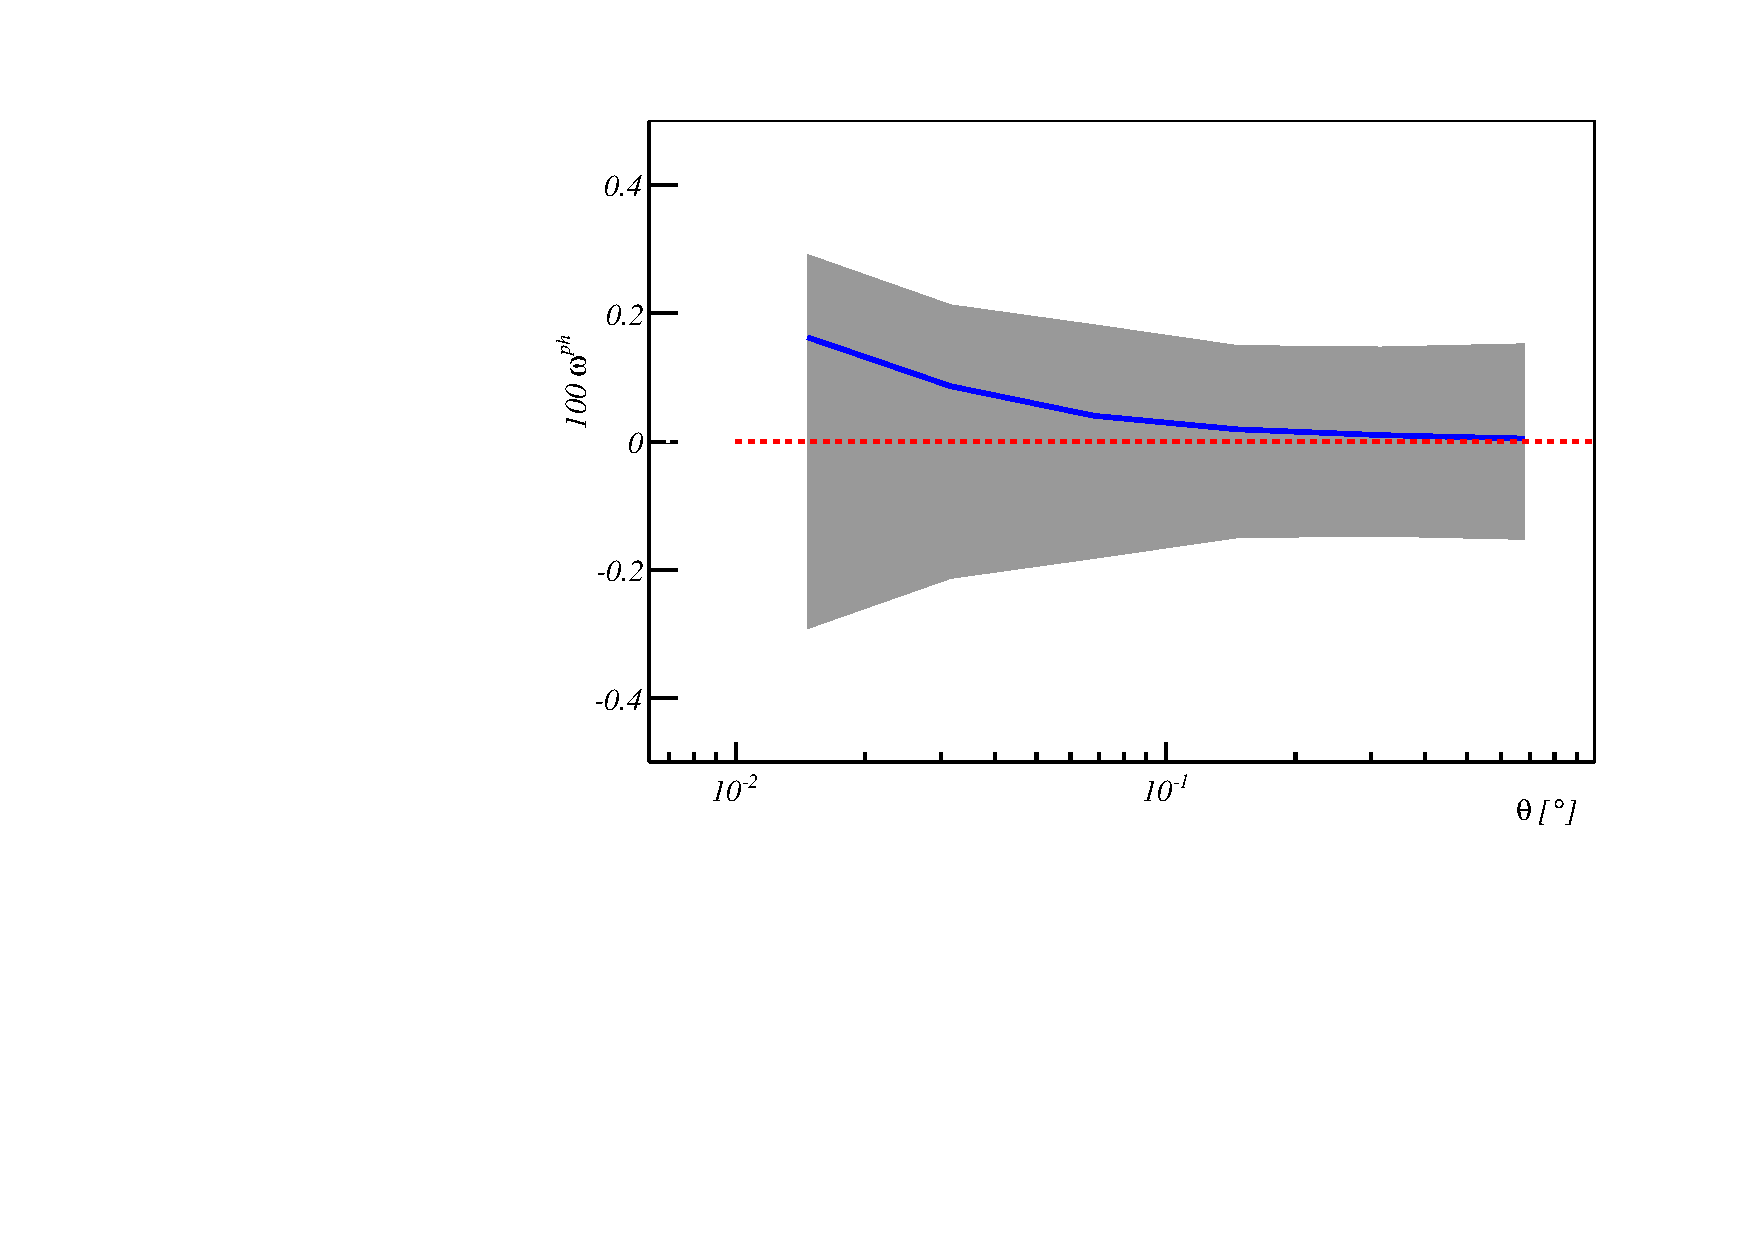
\includegraphics[width=0.5\textwidth]{./figures/mag_itheo_photoz_short.pdf}
\caption{Comparison of $1\sigma$ jackknife errors of the measured correlation function (grey shade) with the expected signal induced by the photo-z migration between the lens and the source sample (sample $I$) computed theoretically with the stacking of the pdfs for the $i$-band (blue line).}
\label{fig:theophotoz}
\end{figure}

A general study of photo-z performance in DES-SV can be found in \cite{2014MNRAS.445.1482S}. A comprehensive study of the photo-z performance and its implications for weak lensing for this data can be found in \cite{PhysRevD.94.042005}. Both studies are followed in this analysis.
\newline
	Conservative photo-z cuts are made in order to minimize migration between lens and source samples. Nevertheless, catastrophic outliers in the photo-z determination can bias the measurement of  $\kappa$ \cite{2010MNRAS.401.1399B}. Thus, the tails of the probability density functions (pdfs) of the photo-z code are a crucial systematic to test.
	\newline
	As mentioned in \autoref{ch:theory}, in addition to the magnification signal, galaxy migration due to a wrong photo-z assignment between lens and source samples may induce a non-zero cross-correlation signal due to the physical signal coming from the clustering of objects in the same redshift bin. As a first approach, estimation of the expected signal induced by photo-z migration ($\omega^{ph}$) is computed with \autoref{eq:4t}:
\begin{equation}
\omega_{\rm LS_j}^{\rm ph}(\theta) = \int\limits_0^\infty dz\int\limits_0^\infty dz' \phi_{\rm L}(z)\phi_{\rm S_j}(z')\xi(\theta;z,z'),
\label{eq:phth}
\end{equation}
where $\xi(\theta;z,z')$ is the 3D correlation-function and $\phi_{\rm L},\phi_{\rm S_j}$ are the redshift distribution of the lens (L) sample and the source sample ($\rm S_j$) estimated from the stacking of the pdfs given by TPZ. \autoref{fig:theophotoz} compares the measured two-point angular cross-correlation and the expected signal induced by photo-z can be seen for the \textit{I} sample. The signal induced by photo-z is found to be smaller than the statistical errors. Note that this method relies on an assumed cosmology and bias model, and therefore should be considered only an approximation. A more accurate calculation can be made with the help of N-body simulations.
\newline

From the overlap of the redshift distribution of both lens and source samples, it is found that the total photo-z migration between lens and source sample is $o\sim 0.6\%$ depending on the magnitude cut of the source sample. The procedure to compute this overlap is to integrate the product of the pdfs of the lens and source sample:
\begin{equation}
o = \int\limits_0^\infty dz\phi_L(z)\phi_S(z),
\end{equation}
where $\phi_L,\phi_S$ are the stacked pdfs of the lens and source sample respectively. Since TPZ provides an individual pdf for each galaxy, the stacked pdf of a given sample is computed by adding all the individual pdfs of the galaxies that belong to that sample (see \cite{2016MNRAS.459.1293A} for a study of clustering with stacked pdfs).
\newline

To estimate the maximum photo-z migration allowed between the lens and the source sample, the MICE simulation (\autoref{sec:mice}) with the un-lensed coordinates and magnitudes is used. Galaxies are randomly sampled on the lens redshift bin and then placed on the source redshift bin. Conversely, galaxies on the source redshift bin are randomly sampled and placed on the lens redshift bin. For a given lens or source sample, the number of galaxies introduced from the other redshift bin is chosen to be 0.1, 0.3, 0.5, 0.7, 0.9 and 2 per cent of the galaxies. Then, the two-point angular cross-correlation is computed for each case. The difference of the correlation functions measured at the simulation with induced migration between lens and source sample and the original used in \autoref{sec:mice} is the signal induced by photo-z migration. The signal induced by photo-z for the cases with 0.9 and 2 per cent computed with this method can be seen at \autoref{fig:photozcontamination}. It is found that  at 0.9 per cent of contamination, the induced signal due to photo-z migration is comparable to the error in the correlation functions. This upper limit is greater than the estimated photo-z migration, demonstrating that the effect of photo-z migration is negligible. Photo-z migration has a larger impact on the brightest samples. Nevertheless, since the errors of the correlation functions of these samples are shot-noise dominated, the tightest constrains on photo-z migration are imposed by the faintest samples. With a larger data sample this statement will no longer be true.
\begin{sidewaysfigure}
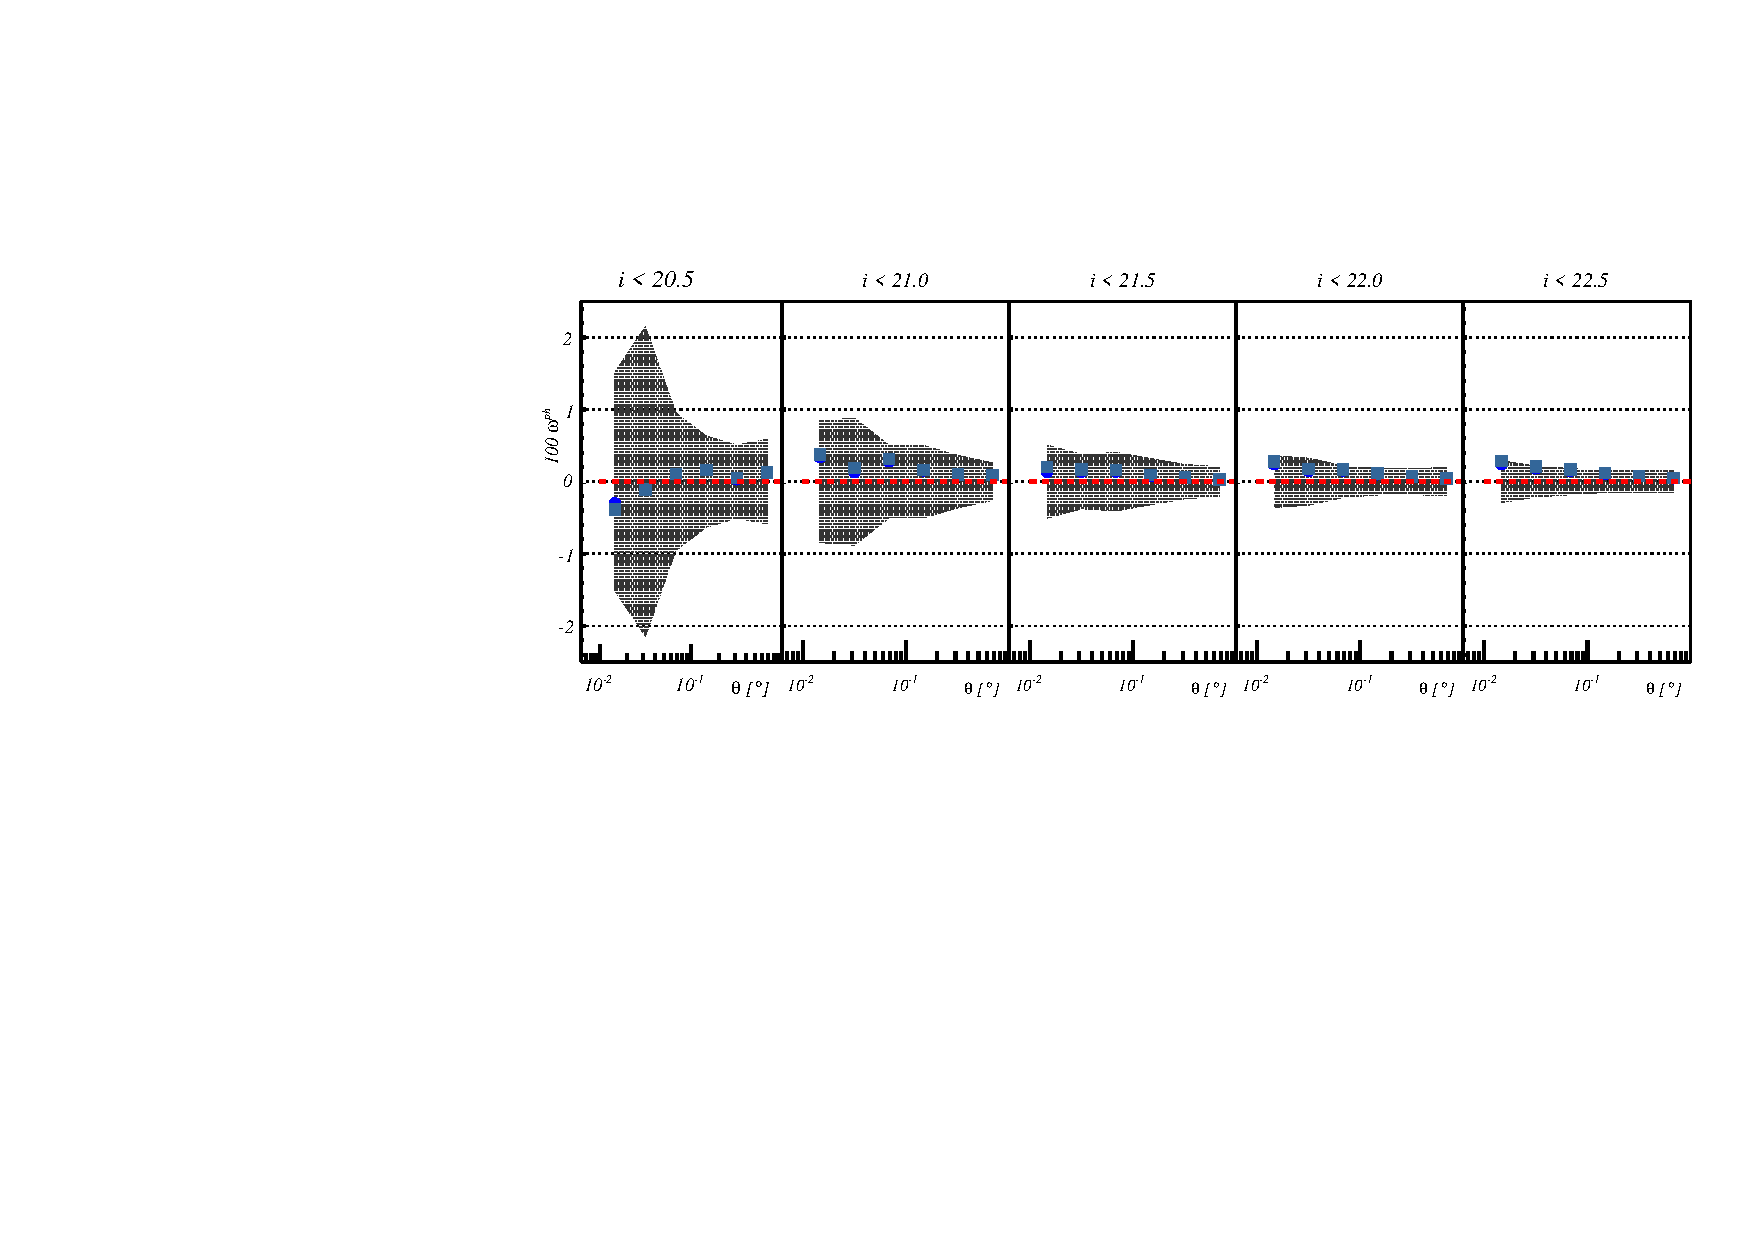
\includegraphics[width=\textwidth,trim={0 2.3cm 0 3.5cm},clip]{./figures/mag_i_mix.pdf}
\caption{Estimation of the signal induced by migration of selected fractions of MICE un-lensed galaxies between the lens and the source sample (sample $I$). Shaded area is the $1\sigma$ confidence interval for the measured number count cross-correlations. Dark blue dots correspond to a contamination fraction of 0.9 per cent. Violet squares correspond to a 2 per cent. Squares are displaced at the X axis for clarity. Red dashed line is an eye-guide for zero.}
\label{fig:photozcontamination}
\end{sidewaysfigure}
\newline

Photo-z induced correlation functions that mimic magnification may affect the measured significance. Thus, Bayes factor is recomputed with two new hypothesis, the measured signal is a combination of magnification and photo-z ($M+Ph$) or the measured signal is only photo-z ($Ph$):
\begin{equation}
\mathcal{B} = \frac{P(M+Ph|\Theta)}{P(Ph|\Theta)} = \frac{P(\Theta|M+Ph)}{P(\Theta|Ph)},
\end{equation}
where
\begin{equation}
P(\Theta|M+Ph) = e^{-\chi^2_{\rm Planck+Ph}/2}
\end{equation}
and
\begin{equation}
P(\Theta|Ph) = e^{-\chi^2_{\rm Ph}/2}.
\end{equation}
To compute $\chi^2_{\rm Planck+Ph}$ and $\chi^2_{\rm Ph}$ it has been assumed that the expected theory is given by $\omega_{\rm LS_j}(\theta)+\omega_{\rm LS_j}^{\rm ph}(\theta)$ and $\omega_{\rm LS_j}^{\rm ph}$ respectively, where $\omega_{\rm LS_j}^{\rm ph}$ is the expected signal induced by photo-z computed using \autoref{eq:phth}. The significances recomputed using these two new hypothesis for the {\it r}, {\it i} and {\it z} bands are $\log_{10}\mathcal{B}=2.5, 4.0, 3.5$ respectively. Thus, it can be concluded that photo-z migration has a limited impact on the measured significances.
\newline

All previous calculations were based on the assumption that the pdfs are a reliable description of the true redshift distribution. This statement can be partially validated comparing the pdfs with the spectroscopic redshift distribution for the same sample (see \autoref{fig:specphotoz} for an example).  Redshift distributions predicted by TPZ are found to be representative of those given by the spectroscopic sample. Nevertheless, this statement has limitations --but is good enough for SV data-- and a more accurate description of the real redshift distribution of the full sample will be measured with methodologies involving clustering-based estimators \cite{2008ApJ...684...88N,2010ApJ...721..456M,2013arXiv1303.4722M,2016MNRAS.462.1683S} when the size of the data sample grows. This type of estimators involve the use of two-point angular cross-correlations between different redshift bins, whose measurement may be biassed by number count magnification itself. Nevertheless, as it has been stated in \autoref{ch:theory}, depending on the value of the number count slope, the amplitude induced by magnification on the correlation-function may be zero. Thus, when employing this kind of estimators, samples should be carefully chosen so that $\alpha_S-1=0$. This can be done by measuring the number count slope at the cumulative magnitude distribution with methods such that used in this work.
\begin{figure}
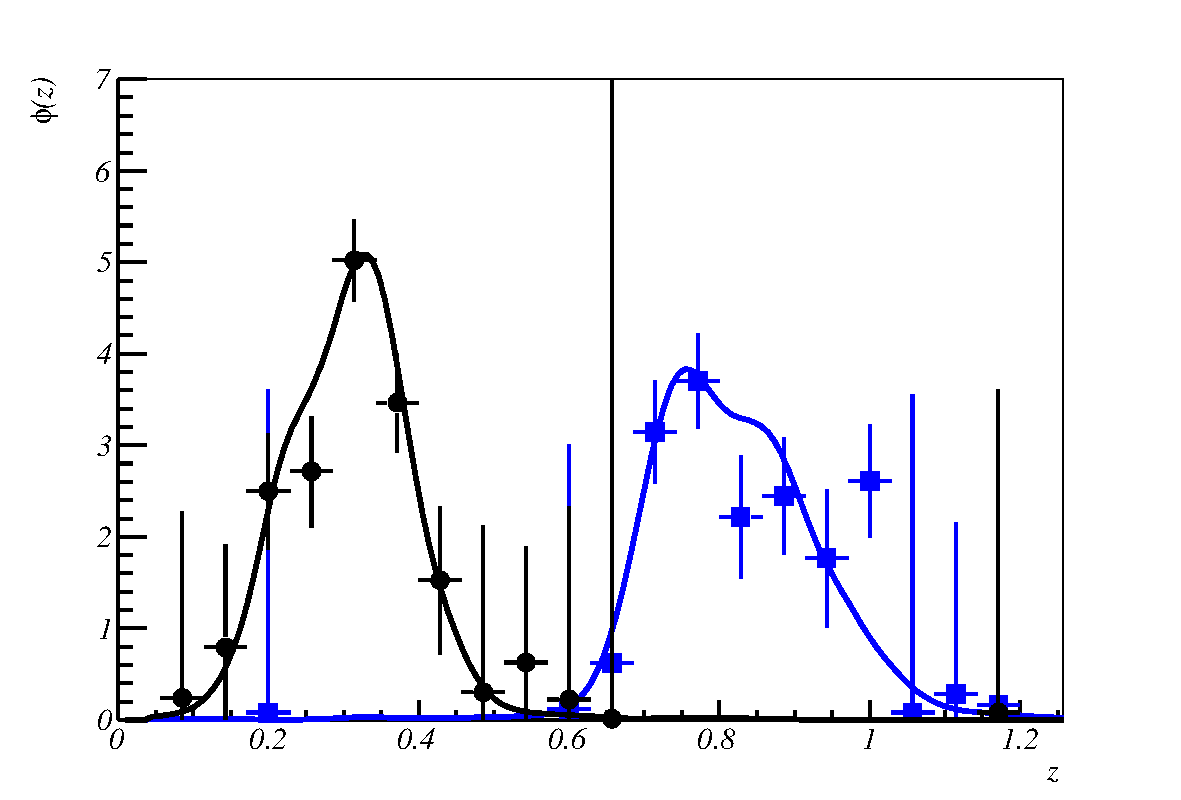
\includegraphics[width=\textwidth]{./figures/spec_photoz_cmp.pdf}
\caption{Comparison of the redshift distribution computed by the stacking of the pdfs given by TPZ ( solid lines) with the ones computed with the spectroscopic sample of the lens (black dots) and the source sample $i<22.5$ (blue squares).}
\label{fig:specphotoz}
\end{figure}
\newline

    Finally, to demonstrate that the measured signal is independent of the photo-z technique employed to estimate the redshift, the two-point angular cross-correlation functions used on this analysis are re-computed with redshift estimated with other two different approaches that have shown to have similar performance as TPZ \cite{2014MNRAS.445.1482S} a neural network, Skynet  \cite{2014MNRAS.441.1741G}, and a template based approach, Bayesian Photo-Z (BPZ) \cite{2000ApJ...536..571B}. \autoref{fig:bpzskynet} compares the cross-correlations computed with the three codes for the $i$-band, showing them to be within $1\sigma$ errors.
\begin{sidewaysfigure}
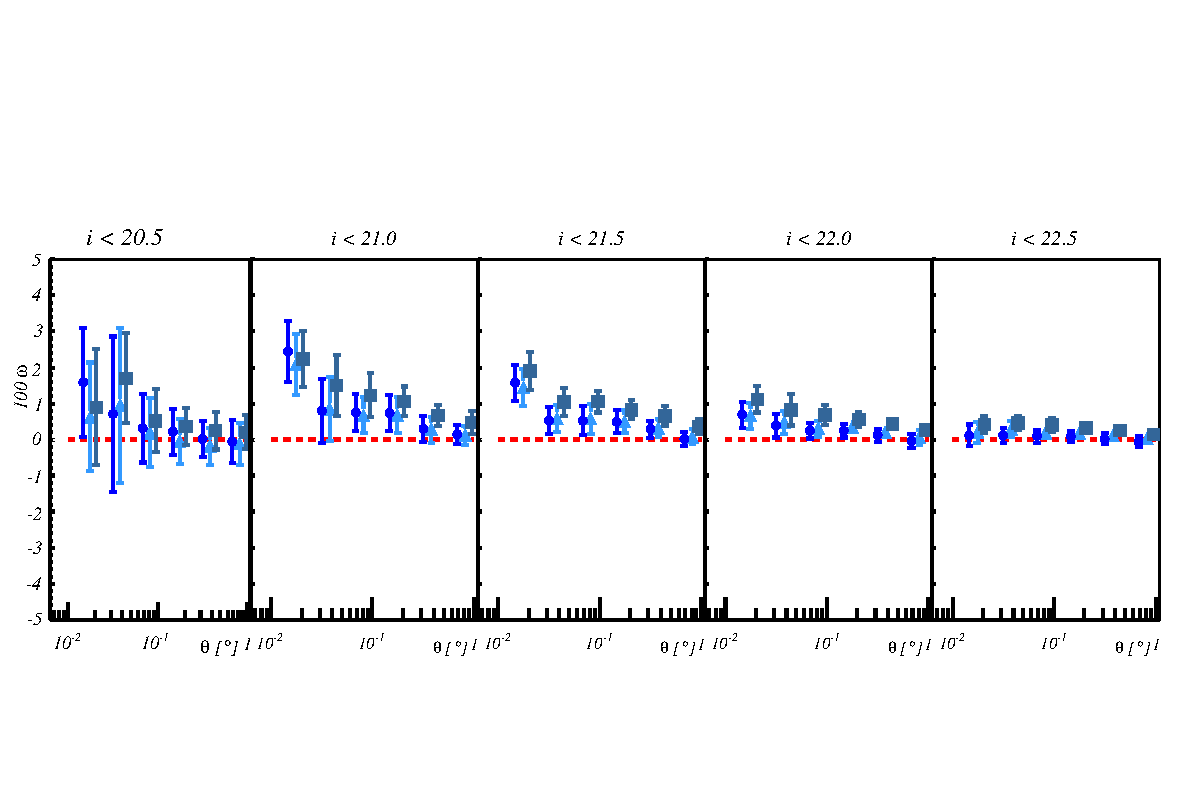
\includegraphics[width=\textwidth,trim={0 2.3cm 0 3.5cm},clip]{./figures/mag_i_photoz_comparison.pdf}
\caption{Comparison of the measured two-point angular cross-correlation functions corresponding to the sample $i<21.5$ measured with the Landy-Szalay estimator using TPZ, Skynet and BPZ. Triangles and squares are displaced at the horizontal axis for clarity.}
\label{fig:bpzskynet}
\end{sidewaysfigure}

\subsection{Discussion}
\label{sec:discussion_sv}

On this analysis, the weak-lensing magnification signal has been detected on the DES-SV data using the general population of galaxies. In addition, a thorough and detailed study of the possible systematic effects is made. The systematic error estimation has been made, for the first time, with the help of two simulations: MICE --a N-body-- and {\scshape Balrog} --an image simulation--.
\newline

From all of the systematic error estimation, two of them have shown to be critical for magnification on photometric surveys: the observing conditions and the photo-z migration between the lens and the source sample.
\newline

This analysis demonstrates that reliable weak-lensing magnification can be measured accurately for a galaxy survey such as DES, opening a whole new window to new physic analysis within the experiment.


\section{Magnification in DES Year 1 data}
\label{sec:y1data}
As the new data-release was available --the DES Year 1 (DES-Y1)-- on May 2016, with more area but less depth, the analysis started after this date were performed here. This new data-sample covers more area and has a bigger number of galaxies than DES-SV, allowing to do analyses that were impossible before within the Dark Energy Survey.
\newline

The goal of this analysis is to use the methodology to measure weak-lensing magnification signal developed at \autoref{sec:analysis_sv} to determine the convergence profile of voids and troughs with the DES-Y1 data. Data sample is described at \autoref{sec:data_sample_y1}. Then, the analysis is described \autoref{sec:analysis_y1} following a systematic error study (\autoref{sec:sys_y1}). Finally a discussion on the analysis can be found at \autoref{sec:discussion_y1}.

\subsection{Data sample}
\label{sec:data_sample_y1}
The DES Y1-Gold galaxy catalog, amounts 1600 deg$^2$ divided between several fields that include the supernovae fields, the stripe-82 (S82) and the SPT field (see \autoref{fig:des_y1_coverage}).
\newline

On the DES-Y1 galaxy catalog, the {\scshape redMaPPer} algorithm \cite{2014ApJ...785..104R} is applied to find galaxy-clusters and luminous red galaxies (LRGs) \cite{2016MNRAS.461.1431R,2016ApJS..224....1R} producing the LRG catalog {\scshape redMaGiC}. Using the {\scshape redMaGiC} catalog, two set of independent lenses are produced to measure their convergence profile: voids and troughs.
\newline

The two lenses represent the emptiest regions of the Universe but they are built on a different manner. Voids are defined as the underdensities on the 3D space (ra,dec and redshift) whereas troughs are defined on the 2D matter projection (ra and dec) --that is, redshift integrated--.
\newline

From the main galaxy catalog, a source sample is build, common to both lens samples.

\subsubsection{Lens sample: voids}
Following the same approach employed by Sanchez et~al. on DES-SV \cite{2017MNRAS.465..746S}, the void-finder algorithm is applied to the Y1-{\scshape redMaGiC} catalog, finding 533 voids. From this catalog, the voids with centers on the region
\begin{equation}
-60 < \mbox{ dec [deg]} < -40
\end{equation}
and redshift $z<0.45$ are selected, amounting 193 voids. The spacial distribution of the voids can be seen at \autoref{fig:footprint_voids} whereas the size and underdensity distribution of the voids can be seen at \autoref{fig:prop_voids}

\begin{figure}
\begin{center}
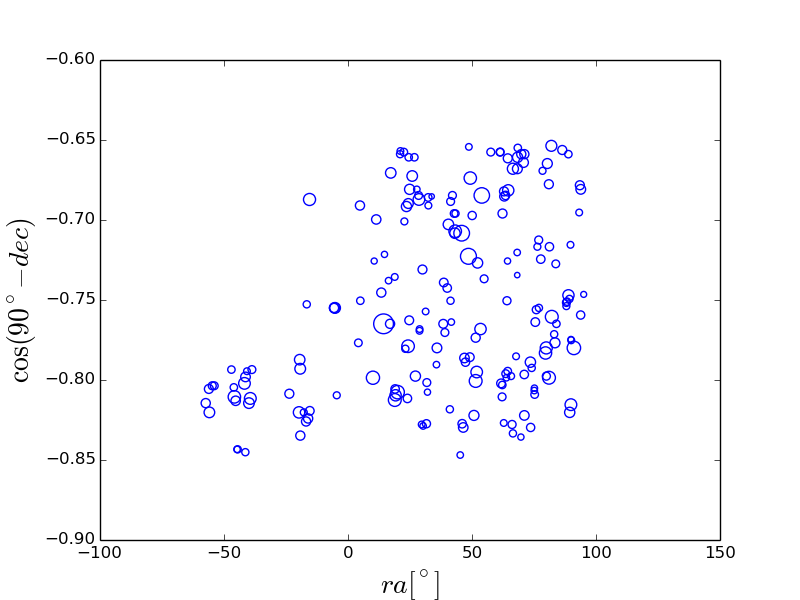
\includegraphics[width=0.85\textwidth]{./figures_y1/voids_footprint.png}
\caption{Spatial distribution of the DES-Y1 voids. The size of the circle is related to the size of the voids.}
\label{fig:footprint_voids}
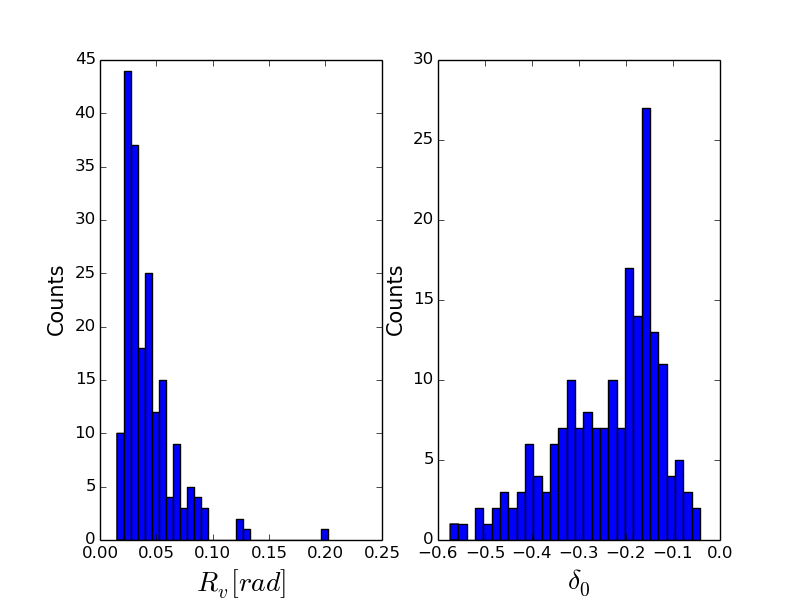
\includegraphics[width=0.85\textwidth]{./figures_y1/voids_prop.png}
\caption{Distributions of the angular size ($R_v$) and central underdensity ($\delta_0$) of the voids.}
\label{fig:prop_voids}
\end{center}
\end{figure}

\subsubsection{Lens sample: troughs}
DES-Y1 troughs have been build following the same approach as on the DES-SV data \cite{2016MNRAS.455.3367G}.

\begin{figure}
\begin{center}
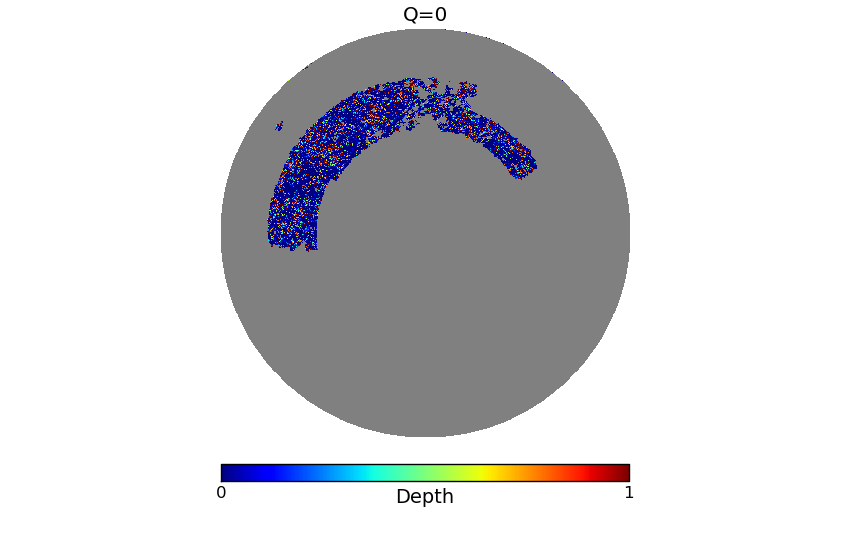
\includegraphics[width=0.49\textwidth,trim={4cm 0 4cm 0},clip]{./figures_y1/trough_10_q0.png}
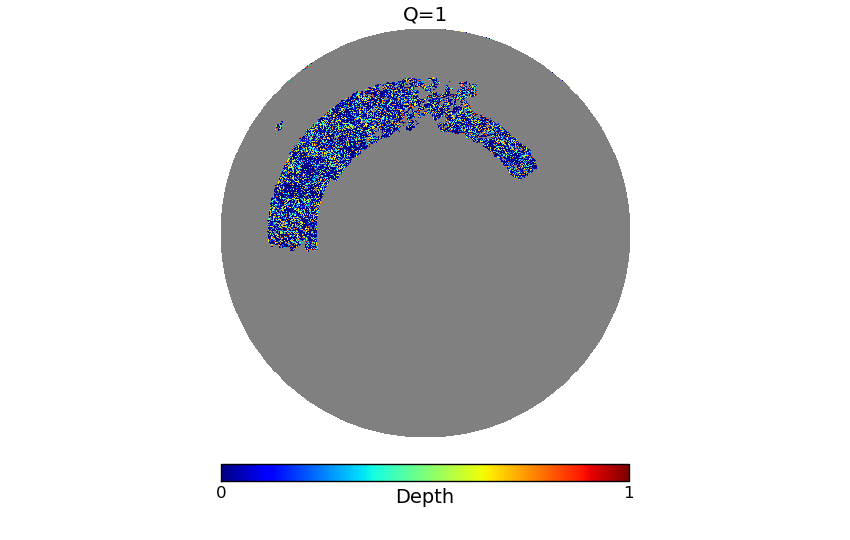
\includegraphics[width=0.49\textwidth,trim={4cm 0 4cm 0},clip]{./figures_y1/trough_10_q1.png}\\
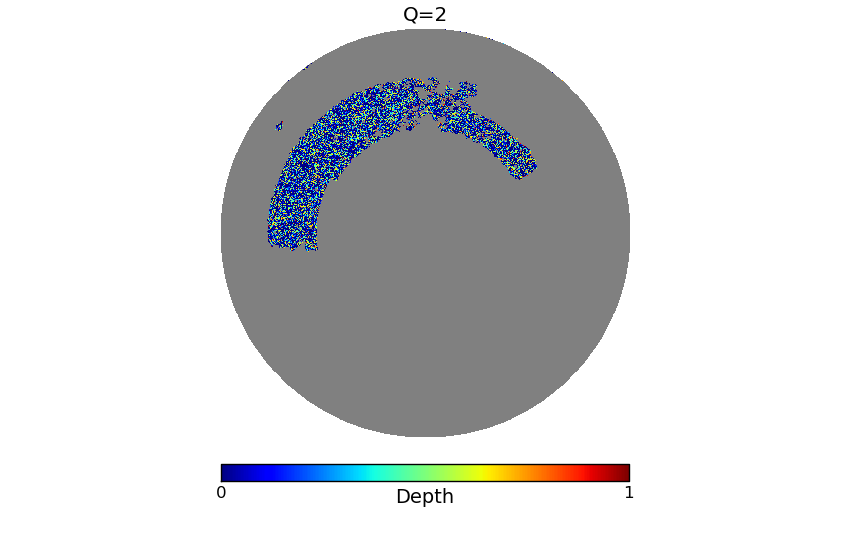
\includegraphics[width=0.49\textwidth,trim={4cm 0 4cm 0},clip]{./figures_y1/trough_10_q2.png}
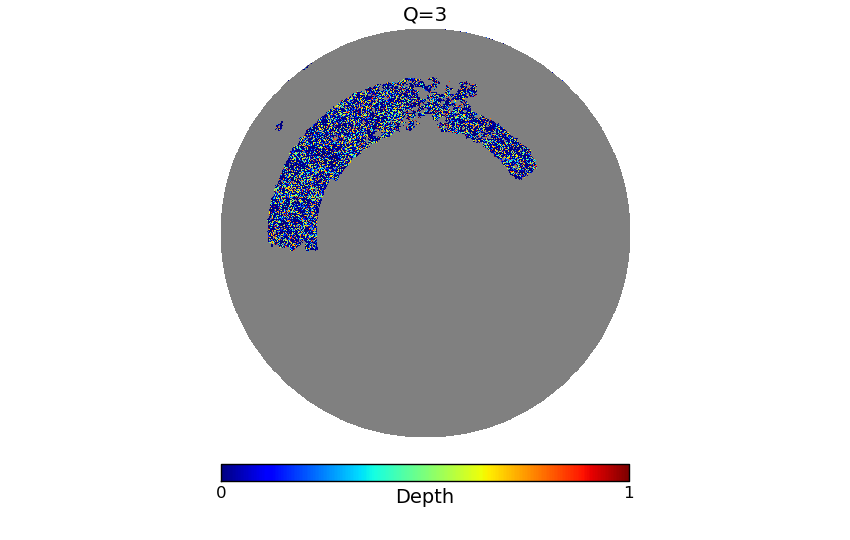
\includegraphics[width=0.49\textwidth,trim={4cm 0 4cm 0},clip]{./figures_y1/trough_10_q3.png}\\
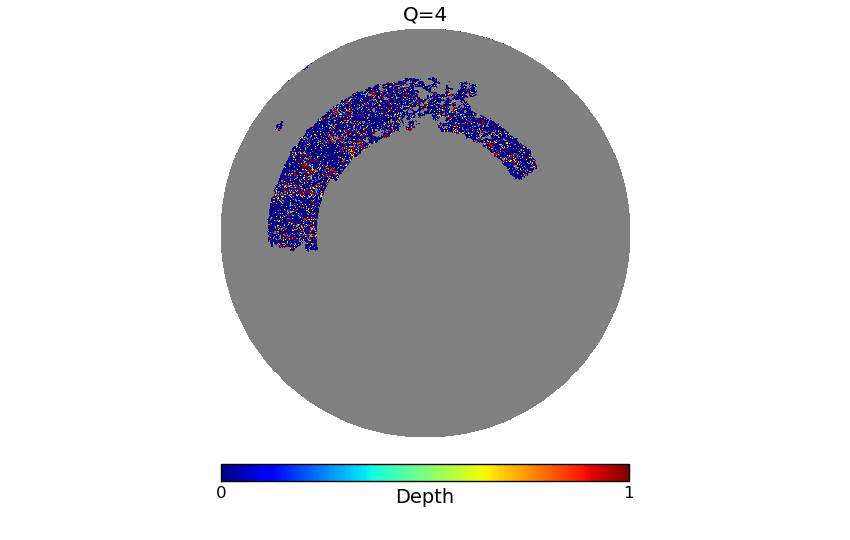
\includegraphics[width=0.49\textwidth,trim={4cm 0 4cm 0},clip]{./figures_y1/trough_10_q4.png}
\end{center}
\caption{{\scshape HEALPix} maps of the $10'$ troughs for the five quantiles considered ($Q$). Orthographic proyection of the Southern Hemisphere cap.}
\label{fig:trough_footprint}
\end{figure}

\subsubsection{Source sample}
From the DES-Y1-Gold main galaxy catalog, the largest contiguous area is selected, the SPT.
\newline

Regions with declination $ < -60^{\circ}$ are removed in order to avoid the Large Magellanic Cloud and severe stellar contamination from the Milky Way. {\scshape Modest\_class} is employed as star-galaxy classifier in combination with the additional morphological cut:
\begin{equation}
\mbox{spread\_model\_i} + \frac{5}{3}\ \mbox{spreaderr\_model\_i} > 0.007.
\end{equation}
\newline

The following color cuts are made in order to remove outliers in color space:
\begin{itemize}
	\item $-1 < g-r < 3$,
	\item $-1 < r-i < 2$,
	\item $-1 < i-z < 2$;
\end{itemize}
where {\it g}, {\it r}, {\it i}, {\it z} stand for the corresponding {\scshape mag\_auto} magnitude measured by {\scshape SExtractor}. Bad regions, and haloes around bright stars are also removed following the same criterias as in \autoref{sec:data_sample_SV}.
\newline

Depth cuts are also imposed on the {\it riz}-bands in order to have uniform depth when combined with the magnitude cuts. These depth cuts are reached by including only the regions that meet the following conditions:
\begin{itemize}
	\item $r_{\rm lim} > 22.5$,
	\item $i_{\rm lim} > 22.0$,
	\item $z_{\rm lim} > 21.0$;
\end{itemize}
where $r_{\rm lim}, i_{\rm lim},z_{\rm lim}$ stand for the magnitude limit in the corresponding band. The resulting footprint, as shown in \autoref{fig:footprint_y1}, after all the masking cuts amounts to $XXXX \mbox{ deg}^2$.
\newline

Photometric redshifts (photo-z) have been estimated using different techniques. In particular, the fiducial code used in this work employs a machine-learning algorithm (random forests) as implemented by TPZ \cite{2013MNRAS.432.1483C}, which was shown to perform well on SV data \cite{2014MNRAS.445.1482S}. The redshifts of the galaxies are defined according to the mean of the probability density functions given by TPZ ($z_{\rm ph}$). Other methods are also employed to demonstrate that the measured two-point angular cross-correlation are not a feature induced by TPZ.
\newline

Three source samples are defined, one per band:
\begin{itemize}
	\item R: $0.7 < z_{\rm ph} < 1.0$ and $r<22.5$;
	\item I: $0.7 < z_{\rm ph} < 1.0$ and $i<22.0$;
	\item Z: $0.7 < z_{\rm ph} < 1.0$ and $z<21.5$.
\end{itemize}

Following the same approach as in the \autoref{sec:svdata}, the {\scshape mag\_auto} cut along with the previously defined depth cuts also guarantee uniformity on the corresponding band. Within each R, I, Z source sample four sub-samples that map the magnitude evolution are defined,
\begin{itemize}
	\item $\rm R_1$: $r<21.0$; $\rm R_2$: $r<21.5$; $\rm R_3$: $r<22.0$; $\rm R_4$: $r<22.5$.
	\item $\rm I_1$: $i<20.5$; $\rm I_2$: $i<21.0$; $\rm I_3$: $i<21.5$; $\rm I_4$: $i<22.0$.
	\item $\rm Z_1$: $z<20.0$; $\rm Z_2$: $z<20.5$; $\rm Z_3$: $z<21.0$; $\rm Z_4$: $z<21.5$.
\end{itemize}
Here $\rm S_j$ with $\rm j=1,2,3,4$ are the sub-samples of sample S with $\rm S\in \{R,I,Z\}$. In \autoref{fig:stacking}, the redshift distributions of the lens and source sample are shown. Note that the sub-samples $\rm R_4, I_4, Z_4$ are equal to $\rm R, I , Z$ respectively.

\subsection{Determination of matter profile: voids \& troughs}
\label{sec:analysis_y1}

\subsection{Systematic errors}
\label{sec:sys_y1}

\subsection{Discussion}
\label{sec:discussion_y1}
